\documentclass{ieeeaccess}
\usepackage{cite}
\usepackage{amsmath,amssymb,amsfonts,amsthm}
\usepackage{mathtools}
\usepackage{graphicx}
\graphicspath{{figs/}{./}}
\usepackage{textcomp}
\usepackage[utf8]{inputenc}
\usepackage[T1]{fontenc}
\usepackage{bm}
\usepackage{algorithm}
\usepackage{algorithmic}
\usepackage{booktabs}
\usepackage{xcolor}
\usepackage{color}
\usepackage{hyperref}
\hypersetup{hidelinks}
\usepackage{multirow}
\usepackage{makecell}
\usepackage{array}
\usepackage{url}
\usepackage{pifont}
\usepackage{siunitx}
\makeatletter
\AtBeginDocument{\DeclareMathVersion{bold}
\SetSymbolFont{operators}{bold}{T1}{times}{b}{n}
\SetSymbolFont{NewLetters}{bold}{T1}{times}{b}{it}
\SetMathAlphabet{\mathrm}{bold}{T1}{times}{b}{n}
\SetMathAlphabet{\mathit}{bold}{T1}{times}{b}{it}
\SetMathAlphabet{\mathbf}{bold}{T1}{times}{b}{n}
\SetMathAlphabet{\mathtt}{bold}{OT1}{pcr}{b}{n}
\SetSymbolFont{symbols}{bold}{OMS}{cmsy}{b}{n}
\renewcommand\boldmath{\@nomath\boldmath\mathversion{bold}}}
\makeatother

% ── Theorem-like environments ──────────────────────────────────────────
\newtheorem{proposition}{Proposition}
\newtheorem{remark}{Remark}
\newtheorem{lemma}{Lemma}
\renewenvironment{proof}{\noindent\textit{Proof.}}{\hfill$\square$\medskip}

% ═══════════════════════ MATH COMMANDS ═══════════════════
\newcommand{\R}{\mathbb{R}}
\newcommand{\SOg}{SO(3)}
\newcommand{\norm}[1]{\left\| #1 \right\|}
\DeclareMathOperator{\atan}{atan2}
\DeclareMathOperator{\Tr}{tr}
\DeclareMathOperator{\Logm}{Log}
\newcommand{\vect}[1]{\bm{#1}}
\newcommand{\mat}[1]{\mathbf{#1}}
\newcommand{\dt}{\Delta t}
\newcommand{\cmark}{\textcolor{black}{\ding{51}}}
\newcommand{\xmark}{\textcolor{black}{\ding{55}}}
% Filled from the N=5 trans/active batteries (scripts/batch_{trans,active}.sh).
\newcommand{\driftPlain}{7}    % plain-EKF hover drift over the transition [%] (7.0+-0.6)
\newcommand{\driftGated}{3}    % gated-EKF held error over the transition [%] (3.3+-0.8)

\begin{document}
\history{Date of publication xxxx 00, 0000, date of current version xxxx 00, 0000.}
\doi{10.1109/ACCESS.2026.0000000}

\title{Identifiability-Aware Virtual Force Sensing and Self-Calibration for Quadrotors}

\author{{Jos\'e Varela-Ald\'as}\authorrefmark{1},~\IEEEmembership{Senior Member, IEEE}, {Ang\'elica Quito}\authorrefmark{2}, {Víctor H. Andaluz}\authorrefmark{3}  and {Alexandre Santos Brandão}\authorrefmark{4},~\IEEEmembership{Member, IEEE}}

\address[1]{Centro de Investigaci\'on MIST, Facultad de Ingenier\'ias,
Universidad Tecnol\'ogica Indoam\'erica, \mbox{Ambato 180103}, Ecuador
(e-mail: josevarela@uti.edu.ec)}

\address[2]{Faculty of Digital Engineering and Emerging Technologies,
International University of Ecuador UIDE, Quito 170411, Ecuador
(e-mail: anquitoca@uide.edu.ec)}

\address[3]{Departamento de Eléctrica, Electrónica y Telecomunicaciones, Universidad de las Fuerzas Armadas ESPE, Sangolquí 171103, Ecuador (e-mail: vhandaluz1@espe.edu.ec)}

\address[4]{Núcleo de Especialização em Robótica, Programa de Pós-Graduação em Ciência da Computação, Departamento de Engenharia Elétrica, Universidade Federal de Viçosa, Viçosa 36570-900, MG, Brazil (e-mail: alexandre.brandao@ufv.br)}

\tfootnote{The research was funded by Universidad Tecnol\'ogica Indoam\'erica.}

\markboth
{J. Varela-Ald\'as \headeretal:~Identifiability-Aware Virtual Force Sensing and Self-Calibration for Quadrotors}
{J. Varela-Ald\'as \headeretal:~Identifiability-Aware Virtual Force Sensing and Self-Calibration for Quadrotors}

\corresp{Corresponding author: Jos\'e Varela-Ald\'as (e-mail: josevarela@uti.edu.ec).}

\begin{abstract}
Many aerial tasks, such as flying in wind or carrying a payload, require the
external force on the airframe, yet quadrotors rarely carry a force sensor. We turn
the onboard inertial measurement unit into a \emph{virtual force sensor}: the
external specific force is read directly from the accelerometer residual. The
obstacle is calibration, since the reading needs the vehicle mass, which is
unidentifiable near hover, where a mass error is indistinguishable from a vertical force; a
standard extended Kalman filter then corrupts the mass. We make the sensor
\emph{identifiability-aware and self-calibrating}. An online identifiability
measure, the Fisher information on the mass, gates the calibration and freezes
the mass when it cannot be seen; and when the flight lacks the excitation to
recalibrate, the controller injects a minimal probe that the same measure
shapes. In simulation the sensor reads the external force with a per-axis
correlation of \num{0.93} under continuous wind; the gate holds the mass
calibration to \SI{3}{\percent} through a windy hover where an ungated filter
drifts to \SI{7}{\percent}; the probe recovers the mass from a wrong prior that
hover alone cannot identify; and feeding the sensed force to a model-predictive
controller reduces the tracking error by \SI{34}{} to \SI{80}{\percent} under
wind, most where the wind dominates the dynamics. The sensor degrades gracefully
under injected accelerometer and thrust errors and runs in real time at
\SI{100}{\hertz}.
\end{abstract}

\begin{keywords}
Aerial robotics, force estimation, inertial sensing, identifiability,
self-calibration, virtual sensors.
\end{keywords}

\titlepgskip=-21pt

\maketitle

% ════════════════════ INTRODUCTION ════════════════════
\section{Introduction}\label{sec:intro}

\PARstart{T}{he} external force acting on a quadrotor, from wind, a payload, or physical
contact~\cite{abbas2026trajectory,aliyu2022control,ding2023adaptive}, governs how it must be flown, yet small aerial platforms rarely carry a
force or wrench sensor: the payload and power budget favor reusing the sensors
already on board. The accelerometer offers a route. It measures the
non-gravitational specific force directly, so once gravity and the commanded
thrust are removed, what remains is the external specific force. This turns the
inertial measurement unit (IMU) into a \emph{virtual force sensor}, with no added
hardware, and the reading is instantaneous: no double-differentiation of position,
no estimator lag.

The virtual sensor has one calibration parameter, the vehicle mass, which converts
the measured acceleration into the thrust contribution that must be subtracted.
The mass is rarely measured online, it is copied from a datasheet or changed by a
payload, and a few-percent error biases the reading. Worse, the mass is only
\emph{conditionally identifiable}: the mass enters the reading only through the
thrust-to-weight ratio, so in near-hover flight a mass error is indistinguishable
from a vertical external force, and an estimator that calibrates it unconditionally
corrupts the very reading it supports. A virtual force sensor for aerial use therefore needs
to know \emph{when} its calibration is reliable and to be able to recalibrate
itself when it is not. That is the problem we address.

Online parameter identification for aerial robots has been studied with
maximum-likelihood frameworks~\cite{burri2018system} and with recursive
regression on inertial signals that recover the mass and inertia under physical
consistency constraints~\cite{wuest2019online,wensing2017geometric}, and with
sparse-regression models identified from flight data for predictive
control~\cite{guevara2025sindy}; these
methods need excited flight to identify the inertial parameters. External-force
estimation has a parallel line of work based on momentum
observers~\cite{tomic2017external,ruggiero2014impedance,yuksel2014nonlinear,guevara2024estimation}, which estimate the
force on the airframe from the dynamics but are biased by errors in the same
parameters above. Moving-horizon estimation has been applied to quadrotor system
identification~\cite{wang2023neuromhe}, building on the constrained-MHE
theory~\cite{rao2003constrained}; the unmodeled aerodynamics that learned
residual models capture are themselves an active
area~\cite{bauersfeld2021neurobem,torrente2021data}. On the control side,
adaptive and incremental schemes reject disturbances without an explicit force
estimate~\cite{smeur2016adaptive,hanover2022performance,chen2016disturbance,zhang2024enhanced,liu2023adaptive}, and learning-based adaptive controllers fit a
disturbance representation online to reject wind in agile
flight~\cite{oconnell2022neuralfly}. These methods cancel the disturbance but do
not reason about \emph{when} the underlying parameters are identifiable.

Two themes run through this work. First, the mass is recoverable only under
sufficient excitation, a persistency-of-excitation condition that classical
optimal input design addresses by shaping the input to maximize the information
about the unknown~\cite{mehra1974optimal}. Freezing a parameter update when it is
not persistently excited is itself classical in adaptive estimation, in the form
of dead-zone and covariance-management schemes~\cite{ioannou1996robust,narendra1987persistent}, and
exciting the input to restore information is classical optimal input
design~\cite{mehra1974optimal}. Our contribution is not either element alone
but the signal that drives both: unlike a dead-zone keyed to a generic
excitation proxy, and unlike a momentum observer that estimates the force without
quantifying its identifiability, we gate on the closed-form Schur complement, which
(i) isolates exactly the mass--vertical-force coupling, (ii) is the marginal Fisher
information on the mass (its inverse is the Cram\'er--Rao bound), and (iii), in its
dimensionless form $\tilde\sigma$, doubles as the
controller's trigger to restore identifiability.
Table~\ref{tab:related} makes the comparison explicit: for each family of
methods it lists what is measured, which signal (if any) decides whether the
parameter is updated, whether the method isolates the mass--vertical-force
coupling, and whether it acts to restore identifiability when the flight does not
provide it. Extended-state and disturbance observers~\cite{han2009pid,chen2016disturbance}
estimate a lumped disturbance with the model, and hence the mass, assumed
known: their disturbance state is the same residual our force reading is built
on, so what we add is not a different observer but the calibration layer around
it, which decides online whether the mass that scales the residual can be
trusted and acts when it cannot; dead-zone and covariance-management schemes~\cite{ioannou1996robust,narendra1987persistent}
stop the update on a generic excitation proxy that cannot tell hover from a
maneuver (Section~\ref{sec:results}); Fisher-optimal input
design~\cite{mehra1974optimal,morelli2022inertia} and dual
control~\cite{mesbah2018dual} plan the excitation offline or implicitly in the
cost; and recursive inertial identification~\cite{wuest2019online,burri2018system,boyacioglu2023inertial}
assumes excited flight. None of them evaluates online, from a closed-form
signal, whether the mass is currently separable from the vertical force, and
none uses that signal both to protect the estimate and to trigger the excitation.
Second, the external force and the inertial parameters are coupled, so estimating
them jointly can bias both. The near-hover mass--vertical-force degeneracy we use
is a known structural fact in aerial estimation; existing methods, to our
knowledge, do not quantify it online to decide \emph{when} a parameter is
reliable or to \emph{act} so that it becomes identifiable. In near-hover flight
the mass and the vertical external force enter the dynamics through the same
channel and are not jointly identifiable, so an estimator that updates both
distributes the error between them. This is the property we exploit.

This paper builds an identifiability-aware, self-calibrating virtual force sensor.
The external force enters the accelerometer almost algebraically, so the sensor
reads it accurately once the mass is calibrated; the mass, by contrast, is only
conditionally identifiable and is confounded with a vertical force near hover. We
make the calibration identifiability-aware on two levels. An extended Kalman filter
(EKF) monitors an online identifiability measure and freezes the mass calibration
when the parameter is unidentifiable, protecting the reading during hover where a
naive filter drifts. When the mass must be recalibrated but the flight is too
weakly exciting to reveal it, the model-predictive controller injects a minimal
\emph{probe}, a small bounded excursion of the position reference (not a sensor),
that restores identifiability and then stops, so the sensor never relies on a
parameter it cannot see. The resulting loop and the role of the identifiability
signal $\tilde\sigma$ are shown in Fig.~\ref{fig:system}.

\begin{table*}[t]
\centering
\caption{Handling of the calibration parameter's identifiability in related
approaches. ``Gate signal'' is what decides whether the parameter is updated;
``$m$--$d_z$'' asks whether the method isolates the mass--vertical-force
coupling; ``restores'' asks whether it acts to recover identifiability.}
\label{tab:related}
\small
\begin{tabular}{lllcc}
\toprule
Approach & What it measures & Gate signal & $m$--$d_z$ & restores \\
\midrule
Momentum / IMU-residual obs.~\cite{tomic2017external,ruggiero2014impedance} & external force ($m$ assumed) & none & no & no \\
ESO / disturbance obs.~\cite{han2009pid,chen2016disturbance} & lumped disturbance ($m$ assumed) & none & no & no \\
Dead-zone, cov.\ management~\cite{ioannou1996robust,narendra1987persistent} & parameter error & generic PE proxy & no & no \\
Fisher-optimal input design~\cite{mehra1974optimal,morelli2022inertia} & information of a planned input & offline & no & offline \\
Dual / active-learning MPC~\cite{mesbah2018dual} & expected future information & implicit (cost) & no & implicit \\
Recursive inertial ID~\cite{wuest2019online,burri2018system,boyacioglu2023inertial} & inertial set, excited flight & none & partial & no \\
\textbf{This work} & $\sigma$ = marginal Fisher info.\ on $m$ & $\tilde\sigma$, online, closed form & yes & online \\
\bottomrule
\end{tabular}
\end{table*}

\begin{figure}[t]
\centering
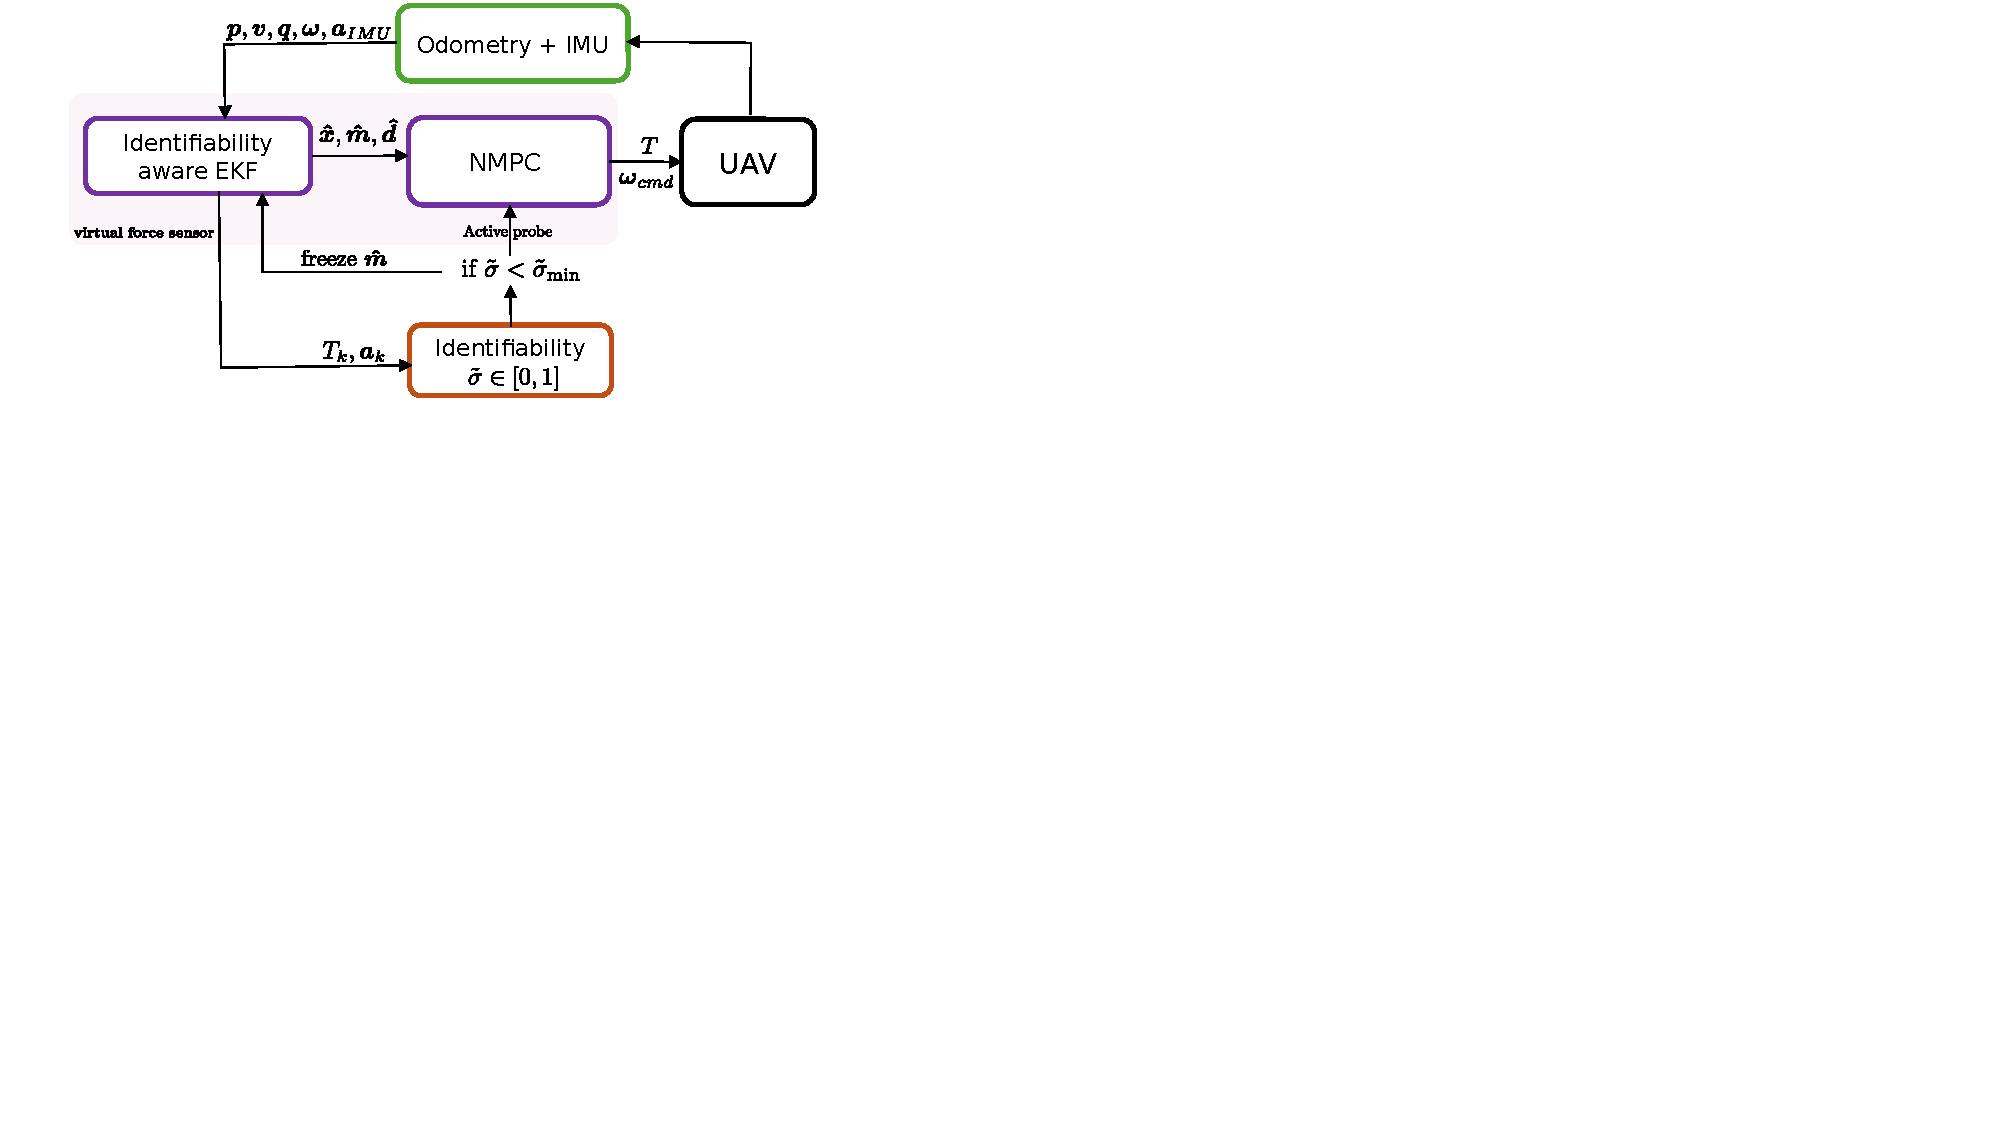
\includegraphics[width=\columnwidth]{figs/fig_system.pdf}
\caption{Architecture of the self-calibrating virtual force sensor: the
identifiability signal gates the mass calibration and triggers the
active probe; the NMPC feeds the estimated force forward.}
\label{fig:system}
\end{figure}

The contributions of this work are the following. The bare reading of the external
specific force from the accelerometer residual is a known momentum/IMU-residual
technique~\cite{tomic2017external,ruggiero2014impedance,smeur2016adaptive}; our
contribution is the identifiability-aware self-calibration layer that makes such a
virtual force sensor reliable on a vehicle whose calibration parameter is only
conditionally identifiable.
\begin{itemize}
\item We give the identifiability analysis of the sensor's calibration: the mass and
the vertical external force are not jointly identifiable in near-hover flight, and we
derive an online identifiability measure, the Schur complement of the force block
in the thrust--acceleration regressor Gramian, which is the marginal Fisher
information on the mass (its inverse is the Cram\'er--Rao bound) and quantifies when
the calibration is reliable.
\item We make the sensor \emph{self-calibrating}. The EKF gates the mass
calibration by this measure, with an explicit quantitative criterion, the
normalized Schur complement falling below a threshold
($\tilde\sigma<\tilde\sigma_{\min}$, \eqref{eq:gate}), freezing the mass when it is
unidentifiable so the reading is protected during hover; and when the mass must be recalibrated but the flight
lacks sufficient excitation, the controller injects a probe to restore
identifiability. The same
$\tilde\sigma$ \emph{shapes} the probe, since maximizing it selects the
most informative excitation within the probe family, so a single identifiability
scalar governs gating, triggering, and excitation design.
\end{itemize}
The resulting sensor is characterized and validated end to end in
software-in-the-loop: it matches the simulator ground truth to about
\SI{0.4}{\newton} RMS per axis (per-axis correlation \num{0.93} under continuous
wind), a moving-horizon estimator does not improve on it because the reading is
algebraically identifiable, and feeding the sensed force to a model-predictive
controller reduces the tracking error by \SI{34}{} to \SI{80}{\percent} under
wind, in real time at \SI{100}{\hertz}.

This is a methodology and feasibility study in software-in-the-loop. We exercise
the sensor against injected accelerometer bias, scale-factor, and thrust-mismatch
errors to probe the dominant real-sensor effects, but a full hardware demonstration,
on a real IMU and thrust map, or on a manipulator whose joint-torque readings give
the same identifiability structure, is the natural next step and is deliberately left
to a dedicated follow-up.

The rest of the paper is organized as follows. Section~\ref{sec:model}
presents the translational model and the measurement equations.
Section~\ref{sec:obs} analyzes identifiability and derives the hover ambiguity and
the identifiability measure. Section~\ref{sec:mhe} describes the
identifiability-aware EKF and its mass gate. Section~\ref{sec:nmpc} presents the
disturbance-rejecting controller and the active excitation.
Section~\ref{sec:setup} reports the experimental setup and
Section~\ref{sec:results} the results. Section~\ref{sec:conclusion} concludes the paper.

% ════════════════════ SYSTEM MODEL ════════════════════
\section{System Model}\label{sec:model}

We model the quadrotor as a rigid body and estimate only its translational
motion. The attitude is measured by the onboard estimator and enters the model
as a known input, which removes the orientation states from the estimator and
keeps it well-conditioned.

\subsection{Frames and notation}
Let $\mathcal{F}_W=\{O_W,\vect{x}_W,\vect{y}_W,\vect{z}_W\}$ be the inertial
world frame and $\mathcal{F}_B=\{O_B,\vect{x}_B,\vect{y}_B,\vect{z}_B\}$ the body
frame attached to the center of mass (CoM). The position of $\mathcal{F}_B$ with
respect to $\mathcal{F}_W$ is $\vect{p}\in\R^3$ and its velocity is
$\vect{v}\in\R^3$. The orientation of $\mathcal{F}_B$ with respect to
$\mathcal{F}_W$ is the rotation matrix $\mat{R}(\vect{q})\in\SOg$, parameterized
by the unit quaternion
$\vect{q}=[q_0,\ \vect{q}_v^{\!\top}]^{\!\top}\in\mathbb{S}^3$, with
$\mathbb{S}^3\triangleq\{\vect{q}\in\mathbb{H}:\norm{\vect{q}}=1\}$ following the
convention of~\cite{shuster1993survey}. The body attitude rate (body rate for short) $\vect{\omega}\in\R^3$ is
the angular velocity of $\mathcal{F}_B$ with respect to $\mathcal{F}_W$ expressed
in $\mathcal{F}_B$. We write $[\cdot]_\times$ for the skew-symmetric operator
that maps a vector to the matrix form of the cross product. The thrust acts
along $\vect{z}_B$, so its direction in $\mathcal{F}_W$ is
$\vect{a}\triangleq\mat{R}(\vect{q})\,\vect{e}_3$ with
$\vect{e}_3=[0,0,1]^{\!\top}$.

\subsection{Rigid-body dynamics}
The quadrotor is a six-degree-of-freedom rigid body actuated by a collective
thrust $T$ along the body $z$ axis and by an inner-loop body-rate controller. Its
state is the position $\vect{p}$, velocity $\vect{v}$, attitude $\vect{q}$, and
body rate $\vect{\omega}\in\R^3$. The dynamics are
\begin{align}
\dot{\vect{p}} &= \vect{v}, \label{eq:dp}\\
\dot{\vect{v}} &= -g\,\vect{e}_3 + \frac{T}{m}\,\mat{R}(\vect{q})\,\vect{e}_3
                  + \vect{d} - c\,\norm{\vect{v}}\,\vect{v},
                  \label{eq:dv}\\
\dot{\vect{q}} &= \tfrac{1}{2}\,\mat{\Omega}(\vect{\omega})\,\vect{q},
                  \label{eq:dq}\\
\dot{\vect{\omega}} &= \tfrac{1}{\tau_{rc}}\,(\vect{\omega}_{\text{cmd}}-\vect{\omega}),
                  \label{eq:dw}
\end{align}
where $g$ is the gravitational acceleration, $m\in\R_{>0}$ is the mass, and $c$
is a quadratic drag coefficient that lumps the dominant unmodeled
aerodynamics~\cite{sun2022comparative}. The attitude kinematics \eqref{eq:dq} use
the matrix
$\mat{\Omega}(\vect{\omega})=\left[\begin{smallmatrix}0 & -\vect{\omega}^{\!\top}\\[2pt] \vect{\omega} & -[\vect{\omega}]_\times\end{smallmatrix}\right]$,
following the convention of~\cite{shuster1993survey,barfoot2017state}. The body rate follows the
first-order response \eqref{eq:dw} to the commanded rate
$\vect{\omega}_{\text{cmd}}$, with time constant $\tau_{rc}$ for the inner-loop
rate controller, while the collective thrust $T$ is commanded directly. The term
$\vect{d}\in\R^3$, expressed in $\mathcal{F}_W$, is the \textit{external
specific force}, the net external force per unit mass acting at the center of
mass,
\begin{equation}
\vect{d}\triangleq \frac{1}{m}\,\vect{f}_e ,
\label{eq:dfdef}
\end{equation}
where $\vect{f}_e\in\R^3$ is the resultant of the forces that the nominal model
does not represent: aerodynamic effects beyond the drag term, wind, and any
added payload. Equivalently, $\vect{d}$ is the residual between the true
acceleration and the acceleration that gravity and thrust predict in
\eqref{eq:dv}; the experiments set the explicit drag coefficient $c=0$, so $\vect{d}$
also lumps the aerodynamic drag. We treat $\vect{d}$ as quasi-static over the
estimation window in near-hover flight, where the velocity-dependent drag is
negligible and the weight of an added mass and a vertical force become indistinguishable
(Section~\ref{sec:obs}); under fast flight $\vect{d}$ varies with velocity, which
the random-walk process model tracks within its bandwidth. Thus $\vect{d}$ is a
\emph{lumped specific-force residual}: the external force (wind, payload) plus the
lumped aerodynamic drag, the former dominating near hover and the latter growing
with speed. The force estimate is validated against the simulator's external-force
channel, and the residual drag is what the random-walk bandwidth limits at high
speed (Section~\ref{sec:results}). The quantities
estimated online are the mass $m$ and the external force $\vect{d}$, which enter
the translational dynamics \eqref{eq:dv}; the rate-loop constant $\tau_{rc}$ is a
nominal known constant of the inner loop, not estimated. To be explicit about
what the sensor relies on: $g$ is known; the drag coefficient $c$ is not
identified but set to zero, so that any drag is lumped into $\vect{d}$ and read as
part of the force; $\tau_{rc}$ enters only the controller's prediction model, not
the estimator; the mass is estimated; and the thrust $T$ comes from the
vehicle's thrust map, which is the one calibration the reading depends on and
whose error is characterized in Section~\ref{sec:senserr} (a \SI{10}{\percent}
thrust mismatch couples almost one-to-one into the mass and barely into the
force).

For estimation the attitude is treated as a known input: $\vect{q}$, and hence
the thrust axis $\vect{a}$, are taken from the accurate onboard estimate, so the
estimator integrates only the translational dynamics
\eqref{eq:dp}--\eqref{eq:dv}, with the thrust $T$ as a known input. This avoids the
quaternion states, with their re-normalization and hemisphere bookkeeping, and
keeps the estimator well-conditioned over the window.

\subsection{Measurement model}
The onboard sensors provide several signals at each step: the position and
velocity from odometry, the attitude $\vect{q}$ and the body rate
$\vect{\omega}$ from the inertial estimator and the gyroscope, and the specific
force from the accelerometer. The translational estimator uses two of them and
treats the attitude as an input. The first is the position--velocity
measurement
\begin{equation}
\vect{y} = [\,\vect{p}^{\!\top},\ \vect{v}^{\!\top}\,]^{\!\top}\in\R^6 ,
\label{eq:y}
\end{equation}
provided by the odometry, which is noisy in the simulator. The second is the
accelerometer, which measures the specific force in $\mathcal{F}_B$, the
non-gravitational acceleration sensed by the IMU~\cite{forster2015imu}; rotated into
$\mathcal{F}_W$ with the measured attitude it reads
\begin{equation}
\vect{s} = \mat{R}(\vect{q})\,\vect{a}_{\text{IMU}}
         = \frac{T}{m}\,\vect{a} + \vect{d} - c\,\norm{\vect{v}}\,\vect{v},
\label{eq:imu}
\end{equation}
the non-gravitational part of \eqref{eq:dv}. The attitude $\vect{q}$ enters as
the known input through $\vect{a}=\mat{R}(\vect{q})\,\vect{e}_3$ rather than as a
state to estimate, and the body rate $\vect{\omega}$ is not needed by the
translational estimator. Because the thrust $T$ and the attitude $\vect{q}$ are
known, \eqref{eq:imu} is an algebraic measurement of $\vect{d}$: the
accelerometer residual senses the external force directly, which turns the
estimator into a virtual force sensor.

% ════════════════════ IDENTIFIABILITY ════════════════════
\section{Identifiability and Excitation}\label{sec:obs}

The accelerometer measurement \eqref{eq:imu} relates the unknowns to known
signals, so we analyze when the mass and the external force can be recovered
from it. The drag term is a known function of the measured velocity, so we move
it to the left-hand side and define the compensated specific force
$\tilde{\vect{s}}\triangleq\vect{s}+c\,\norm{\vect{v}}\,\vect{v}$. With the
inverse mass $\beta\triangleq m^{-1}$, \eqref{eq:imu} becomes
\begin{equation}
\tilde{\vect{s}} = T\,\vect{a}\,\beta + \vect{d}
                 = \mat{\Phi}\,\vect{\varphi},
\qquad
\mat{\Phi} = [\,T\vect{a}\ \ \mat{I}_3\,],\quad
\vect{\varphi}=[\beta,\ \vect{d}^{\!\top}]^{\!\top},
\label{eq:regressor}
\end{equation}
which is linear in the unknown $\vect{\varphi}\in\R^4$ with regressor
$\mat{\Phi}\in\R^{3\times4}$. The thrust $T$ and the thrust axis $\vect{a}$ are
known, so identifiability of $\vect{\varphi}$ is the identifiability of
$(m,\vect{d})$.

The accelerometer is what makes \eqref{eq:regressor} algebraic. Without it, the
force $\vect{d}$ would enter only through the velocity derivative
$\dot{\vect{v}}$ in \eqref{eq:dv} and would have to be recovered by
differentiating the noisy odometry twice, which amplifies noise and adds a
delay. Reading $\vect{d}$ from the specific force \eqref{eq:imu} removes that
differentiation and yields an instantaneous algebraic measurement, which is the
basis of the virtual force sensor and decouples the analysis of $\vect{d}$ from
the integration of the trajectory.

The same distinction separates the reading from an energy-based one. With all
parameters known, the work done by the external force is the difference between
the energy delivered by the thrust and the change in the vehicle's kinetic and
potential energy, and it could be read from that balance. But the balance is a
scalar (it loses the direction of the force), it is an integral (the force enters
as $\int\vect{d}\cdot\vect{v}\,dt$, so it lags), and it vanishes wherever the
velocity does, which is exactly the hover where the force matters most. The
specific-force reading \eqref{eq:regressor} is a vector, instantaneous, and
independent of the velocity.

The estimator augments the position and velocity with the mass and the force.
The position and velocity are measured by the odometry \eqref{eq:y} at every step,
so the recoverability of the parameters reduces to the \emph{identifiability} of
$(m,\vect{d})$ from the accelerometer model \eqref{eq:regressor} accumulated over
the window, a persistency-of-excitation condition on the regressor rather than a
full nonlinear observability test of the augmented state. We therefore speak of
\emph{identifiability} throughout: the property in question is that of the
parameters $(m,\vect{d})$ in the regressor, not the observability of the state,
although the two coincide here because the position and the velocity are
measured directly; a nonlinear observability treatment of the inertial
parameters of a rigid body can be found in~\cite{boyacioglu2023inertial}. This
identifiability determines when the mass and the force can be separated and is
what we analyze and exploit.

A single sample gives three equations for four unknowns, so $\vect{\varphi}$ is
recovered only by accumulating samples. Over a window of $N$ samples the
information is the Gramian $\mat{G}=\sum_{k=1}^{N}\mat{\Phi}_k^{\!\top}\mat{\Phi}_k$,
which has the block form
\begin{equation}
\mat{G}=
\begin{bmatrix}
\sum_k T_k^2 & \sum_k T_k\vect{a}_k^{\!\top}\\[2pt]
\sum_k T_k\vect{a}_k & N\,\mat{I}_3
\end{bmatrix},
\label{eq:gramian}
\end{equation}
where $\norm{\vect{a}_k}=1$ was used. The force block $N\mat{I}_3$ is always
nonsingular, so given the mass, $\vect{d}$ is recovered whenever the
window is nonempty; the joint degeneracy that remains is confined to the
mass--vertical-force pair at hover (Proposition~\ref{prop:hover}). The
mass enters only through $\beta$, which is identifiable if and only if the Schur
complement of the force block is positive,
\begin{equation}
\sigma \triangleq \sum_k T_k^2 - \tfrac{1}{N}\,\Big\|\textstyle\sum_k T_k\vect{a}_k\Big\|^2 > 0 .
\label{eq:schur}
\end{equation}
The scalar $\sigma$ is the dispersion of the thrust \emph{vectors} $T_k\vect{a}_k$
about their mean, and it becomes positive through a change in the thrust
magnitude $T_k$, a change in its direction $\vect{a}_k$, or both; it is zero only
when the vectors are identical across the window, which is the case at hover. Its dimension is thrust squared (newtons squared; the italic $N$ denotes the window length), so its
absolute scale grows with the thrust level of the maneuver. To obtain a
dimensionless, maneuver-comparable measure we normalize it by the thrust energy
in the window,
\begin{equation}
\tilde\sigma \triangleq \frac{\sigma}{\sum_k T_k^2}\in[0,1],
\label{eq:snorm}
\end{equation}
the fraction of the thrust energy that lies in the dispersion: $\tilde\sigma=0$
at hover and $\tilde\sigma\!\to\!1$ when the thrust vectors are maximally spread.
Normalizing by the absolute thrust level removes the dominant source of the
threshold's maneuver dependence, so a single $\tilde\sigma_{\min}$ classifies the
regime across maneuvers far better than the raw $\sigma$
(Section~\ref{sec:sens}). The normalization also discards information that the
bound below retains: two windows with the same $\tilde\sigma$ but different thrust
levels, or different accelerometer noise, carry different absolute Fisher
information. We therefore keep the two roles apart throughout: $\tilde\sigma$ is the
dimensionless \emph{classification} signal that decides the regime, and
$\sigma/r_s$ is the \emph{information content} that lower-bounds the variance;
Section~\ref{sec:sens} reports both side by side for every regime flown.

\begin{proposition}\label{prop:hover}
In stationary level hover, where $\vect{a}_k=\vect{e}_3$ and $T_k=\bar{T}$ are
constant over the window, the inverse mass $\beta$ is not identifiable
($\sigma=0$). Equivalently, only the combination $\bar{T}\beta+d_z$ is
identifiable, while $\beta$ and the vertical force $d_z$ are not separately
identifiable.
\end{proposition}
\begin{proof}
With $\vect{a}_k=\vect{e}_3$ and $T_k=\bar{T}$ we have $\sum_k T_k^2=N\bar{T}^2$
and $\sum_k T_k\vect{a}_k=N\bar{T}\vect{e}_3$, so
$\sigma = N\bar{T}^2-\tfrac{1}{N}\,N^2\bar{T}^2 = 0$, and $\beta$ is not
identifiable by \eqref{eq:schur}. The structure is explicit in
\eqref{eq:regressor}: the vertical row reads
$\tilde{s}_z=\bar{T}\beta+d_z$, a single equation in the two unknowns
$\beta$ and $d_z$, whereas the horizontal rows read
$\tilde{s}_{x,y}=d_{x,y}$ since $\vect{a}=\vect{e}_3$. Hence $d_x$ and $d_y$ are
identifiable while $\beta$ and $d_z$ collapse onto their sum.
\end{proof}

\begin{remark}
The ambiguity is confined to the vertical axis and to the pair $(m,d_z)$: a
mass error and a vertical force produce the same accelerometer residual at
hover. The joint ambiguity is confined to the mean thrust direction, which at
and near hover is vertical, so the horizontal components $d_x$ and $d_y$ remain
identifiable there, which is why the external force is recovered in the directions
where wind dominates.
\end{remark}

Away from hover the thrust axis tilts and its magnitude varies, so the vectors
$T_k\vect{a}_k$ disperse and $\sigma>0$; the window is then persistently exciting for
the mass. Since the Cram\'er--Rao lower bound on
the mass estimate scales with $\sigma^{-1}$ (derived in \eqref{eq:crb} below), a
more aggressive trajectory admits a better-conditioned estimate, while the force,
conditioned by the block
$N\mat{I}_3$ given the mass, is read with the same accuracy in every regime with
an accurate held mass. The mass is thus
identifiable under motion and degenerate only at hover, which
Section~\ref{sec:results} confirms by identifying it accurately across the range
of flight speeds.

The scalar $\sigma$ is therefore an online measure of how well the mass can be
identified, read directly from the known thrust and attitude over the window with
no extra sensing. It also has an estimation-theoretic meaning, which we state as
a proposition because the gate and the probe of Section~\ref{sec:nmpc} rest on it.

\begin{proposition}[Cram\'er--Rao bound on the mass]\label{prop:crb}
Let the accelerometer noise be zero-mean with isotropic covariance $r_s\mat{I}_3$
and let $\vect{d}$ be constant over the window. Then the marginal Fisher
information on the inverse mass $\beta$, after profiling out the jointly
estimated force $\vect{d}$, is $\sigma/r_s$, and any unbiased estimate satisfies
\begin{equation}
\mathrm{var}(\hat\beta)\ \geq\ r_s\,[\mat{G}^{-1}]_{11}\,=\,r_s\,\sigma^{-1}.
\label{eq:crb}
\end{equation}
\end{proposition}
\begin{proof}
The joint Fisher information of $(\beta,\vect{d})$ over the window is
$\mat{G}/r_s$, with $\mat{G}$ the Gramian \eqref{eq:gramian}. By the block-inverse
formula, the $(1,1)$ entry of $\mat{G}^{-1}$ is the inverse of the Schur complement
of the force block, $[\mat{G}^{-1}]_{11}=\sigma^{-1}$, and the Cram\'er--Rao
inequality gives \eqref{eq:crb}.
\end{proof}

The bound diverges as $\sigma\to0$ at hover and tightens as the maneuver disperses
the thrust vectors. It is the batch least-squares bound under the stated
assumptions, the limit that the recursive filter approaches under excitation, and
we use it as a relative identifiability measure rather than an absolute
uncertainty. It is stated on the inverse mass $\beta$; since
$\mathrm{var}(\hat m)\approx m^4\,\mathrm{var}(\hat\beta)$ for small errors, the
bound on the mass itself scales with the same $\sigma^{-1}$.

Proposition~\ref{prop:crb} holds $\vect{d}$ constant over the window, whereas the
filter of Section~\ref{sec:mhe} models it as a random walk of per-step variance
$q_d$, and the applied disturbance contains wind steps and, at speed, a
velocity-dependent drag. Under the random-walk model the nuisance is a
trajectory rather than a single vector, and the exact marginal Fisher
information on $\beta$ is a weighted Schur complement
$\sigma_{\mathrm{eff}}\leq\sigma$, derived at the end of this section, which
reduces to $\sigma$ as $q_d\to0$. Section~\ref{sec:sens} evaluates it on logged
flight data: for the implemented $q_d=10^{-2}$, a drift of about
\SI{1}{\meter\per\square\second} per second (half the applied wind), the
information in a \SI{1}{\second} window is \SI{12}{\percent} of the constant-force
value, and the ratio decreases with the window length because a longer window gives
the random walk more freedom to absorb the slow variations of $T\vect{a}$.
Proposition~\ref{prop:crb} is thus an optimistic bound for the implemented
filter; Section~\ref{sec:sens} shows that the random-walk bound accounts for most
of the gap between it and the empirical spread of the estimate. For the
disturbance profiles (steps and sinusoid) and the range of $q_d$ evaluated, the
gate decision is unaffected by the approximation: it thresholds the dimensionless
$\tilde\sigma$ as a regime classifier with an empirical margin, and at hover
$\sigma_{\mathrm{eff}}$ stays at the noise floor for every $q_d$ tested, so the
separation between the regimes survives (Section~\ref{sec:sens}); we did not
sweep the physical bandwidth of the disturbance separately.

\emph{Exact information under the random-walk force model.} Stack the compensated specific forces of the window as
$\vect{S}=[\tilde{\vect{s}}_1^{\!\top},\dots,\tilde{\vect{s}}_N^{\!\top}]^{\!\top}\in\R^{3N}$,
and let $\vect{t}=[T_1\vect{a}_1^{\!\top},\dots,T_N\vect{a}_N^{\!\top}]^{\!\top}$ and
$\mat{M}=[\mat{I}_3,\dots,\mat{I}_3]^{\!\top}\in\R^{3N\times3}$. With the force
evolving as $\vect{d}_k=\vect{d}_{k-1}+\vect{w}_k$,
$\vect{w}_k\sim\mathcal{N}(\vect{0},q_d\mat{I}_3)$, and accelerometer noise
$\vect{n}_k\sim\mathcal{N}(\vect{0},r_s\mat{I}_3)$, the window model
\eqref{eq:regressor} reads
\begin{equation}
\begin{aligned}
\vect{S}&=\vect{t}\,\beta+\mat{M}\,\vect{d}_1+\vect{\epsilon},\qquad
\vect{\epsilon}\sim\mathcal{N}(\vect{0},\mat{\Sigma}),\\
\mat{\Sigma}&=r_s\mat{I}_{3N}+q_d\,\mat{C}\otimes\mat{I}_3,
\end{aligned}
\label{eq:rwmodel}
\end{equation}
with $[\mat{C}]_{kl}=\min(k,l)-1$, where the increments have been marginalized into
the covariance and the initial force $\vect{d}_1$ is a nuisance parameter with a
flat prior. The Fisher information of $(\beta,\vect{d}_1)$ is
\begin{equation}
\mat{J}=
\begin{bmatrix}
\vect{t}^{\!\top}\mat{\Sigma}^{-1}\vect{t} & \vect{t}^{\!\top}\mat{\Sigma}^{-1}\mat{M}\\[2pt]
\mat{M}^{\!\top}\mat{\Sigma}^{-1}\vect{t} & \mat{M}^{\!\top}\mat{\Sigma}^{-1}\mat{M}
\end{bmatrix},
\end{equation}
and the marginal information on $\beta$ is its Schur complement,
\begin{equation}
\begin{aligned}
\frac{\sigma_{\mathrm{eff}}}{r_s}\triangleq{}&
\vect{t}^{\!\top}\mat{\Sigma}^{-1}\vect{t}\\
&-\vect{t}^{\!\top}\mat{\Sigma}^{-1}\mat{M}\,
\big(\mat{M}^{\!\top}\mat{\Sigma}^{-1}\mat{M}\big)^{-1}
\mat{M}^{\!\top}\mat{\Sigma}^{-1}\vect{t}.
\end{aligned}
\label{eq:sigeff}
\end{equation}
For $q_d=0$, $\mat{\Sigma}=r_s\mat{I}_{3N}$ and \eqref{eq:sigeff} reduces to
$\sigma/r_s$ of Proposition~\ref{prop:crb}. For $q_d>0$, $\mat{\Sigma}^{-1}$
down-weights the slow variations of $\vect{t}$, those a random walk can follow, so
$\sigma_{\mathrm{eff}}\leq\sigma$; the fast excitation of the probe is the part
that survives. Evaluating \eqref{eq:sigeff} is a $3N\times3N$ solve,
about \SI{0.7}{\milli\second} at $N=100$ when evaluated numerically, so it could replace $\sigma$ in the
gate; since the gate thresholds the dimensionless ratio with margin, we retain the
closed-form $\tilde\sigma$.

For \emph{gating} we use the dimensionless normalization $\tilde\sigma$
\eqref{eq:snorm}, which normalizes by the thrust level so that a single threshold
$\tilde\sigma_{\min}$ holds across maneuvers; $\sigma$ carries the information
content and $\tilde\sigma$ carries the decision. The threshold is set with margin
between the hover and maneuver values of $\tilde\sigma$ (Section~\ref{sec:sens}),
and Proposition~\ref{prop:crb} translates it into the best resolution that the
admitted data could give. Over a window of $N$ samples near hover thrust,
$\sum_k T_k^2\approx N(mg)^2$, so for a window that just opens the gate,
$\sigma=\tilde\sigma_{\min}N(mg)^2$, the Cram\'er--Rao bound reads
\begin{equation}
\frac{\mathrm{std}(\hat m)}{m}\ \gtrsim\ \frac{1}{g}\sqrt{\frac{r_s}{\tilde\sigma_{\min}\,N}}\,.
\label{eq:thrcrb}
\end{equation}
With the parameters used in the experiments ($\tilde\sigma_{\min}=0.009$,
$N=100$, $r_s=0.5$; Section~\ref{sec:setup}) this is \SI{7.6}{\percent} for one second of data and
\SI{2.4}{\percent} after ten. The bound is a floor, not a guarantee: for a
one-second window at or below the threshold, even an efficient unbiased
estimator could not attain a standard deviation smaller than \SI{7.6}{\percent},
which is of the scale of the \SIrange{5}{7}{\percent} hover bias the gate guards
against (Section~\ref{sec:results}). Under the same ideal constant-force
assumptions, the floor crosses the \SI{3.3}{\percent} residual observed in the
windy hover after approximately \SI{5.3}{\second} of accumulated admissible data
and reaches \SI{2.4}{\percent} after ten seconds. These figures characterize only
the best-case variance permitted by the information; they neither predict nor
upper-bound the realized estimation error. The estimator uses
$\tilde\sigma$ to decide when to trust the mass, and the controller of
Section~\ref{sec:nmpc} uses it to decide when to excite.

Proposition~\ref{prop:hover} has a direct operational reading, summarized in
Table~\ref{tab:obs}. The external force is recoverable in every regime given an
accurate held mass, and is
recovered by any recursive estimator that uses the accelerometer residual; the
mass is recoverable only when the
flight excites it ($\sigma$ large), and is then identified jointly with the
force. This motivates the two elements of our method: an estimator that updates
the mass only when $\sigma$ is large (Section~\ref{sec:mhe}), and a controller
that creates the excitation when the mass must be identified but the flight
lacks the excitation to reveal it (Section~\ref{sec:nmpc}).

\begin{table}[t]
\centering
\caption{Identifiability regimes (Proposition~\ref{prop:hover}). The ``degraded''
$d_z$ entry is the joint case; with an accurate held mass it is recovered
(Section~\ref{sec:results}).}
\label{tab:obs}
\begin{tabular}{lcc}
\toprule
Quantity & Hover & Maneuver \\
\midrule
mass $m$        & unidentifiable ($\sigma\!\approx\!0$)         & identifiable ($\sigma$ large) \\
$d_x,\,d_y$     & identifiable                                  & identifiable \\
$d_z$           & degraded ($m$--$d_z$)                       & identifiable \\
\bottomrule
\end{tabular}
\end{table}

% ════════════════════ ESTIMATOR ════════════════════
\section{Identifiability-Aware Estimation}\label{sec:mhe}

We estimate the translational state and the parameters of
Section~\ref{sec:model} with an extended Kalman filter (EKF) whose state augments
the position and velocity with the mass and the external force,
\begin{equation}
\vect{x}=[\,\vect{p}^{\!\top},\ \vect{v}^{\!\top},\ m,\ \vect{d}^{\!\top}\,]^{\!\top}\in\R^{10}.
\label{eq:state}
\end{equation}
The known inputs at each step are the thrust $T$ and the thrust axis $\vect{a}$.
The position and velocity follow \eqref{eq:dp}--\eqref{eq:dv}, while the mass and
the external force have no dynamics of their own and evolve as random walks with
diagonal process covariance $\mat{Q}=\mathrm{diag}(q_p\mat{I}_3,q_v\mat{I}_3,q_m,q_d\mat{I}_3)$
(Table~\ref{tab:params}). Treating the
attitude as a known input keeps the filter free of quaternion states and their
log-map singularity; the body rate is not needed by the translational estimator.

\begin{table}[t]
\centering
\caption{Estimator and controller parameters.}
\label{tab:params}
\setlength{\tabcolsep}{4pt}
\resizebox{\columnwidth}{!}{%
\begin{tabular}{lll}
\toprule
Block & Parameter & Value \\
\midrule
Plant / sim       & mass, rate $\tau_{rc}^{-1}$    & \SI{1.05}{\kilogram}, \SI{18}{\per\second} \\
Drag              & $c$ (estimator)            & $0$ (lumped into $\hat{\vect{d}}$) \\
Odometry noise    & injected on $p,v$          & MuJoCo, released config \\
Wind              & profile, amplitude         & step / sine, $\sim$\SI{2}{\newton} \\
EKF meas.\ var.   & $r_p,\,r_v,\,r_s$           & $0.02,\ 0.1,\ 0.5$ \\
EKF process       & $q_p,\,q_v,\,q_m,\,q_d$     & $10^{-6},10^{-3},10^{-5},10^{-2}$ \\
Mass gate         & window, dwell $t_d$, $\tilde\sigma_{\min}$ & \SI{1.0}{\second}, \SI{0.25}{\second}, $0.009$ \\
Smoothing         & $\alpha_m,\,\alpha_d$       & $0.995,\ 0.92$ \\
Active probe      & budget $\rho$, $f_\ell$, $f_z$, optimal & \SI{0.80}{\meter}, \SI{0.5}{\hertz}, \SI{1.0}{\hertz}, vertical \\
                  & withdrawal $t_p$ (gate-open time) & \SI{15}{\second} \\
NMPC              & $N_c$, horizon             & $31$, \SI{1.5}{\second} \\
NMPC weights      & $\mat{Q}_p,\mat{Q}_a,\mat{Q}_v$ & $180,\ 20,\ 30$ \\
                  & $\mat{R}_u$                & $\mathrm{diag}(0.3,5,5,5)$ \\
NMPC limits       & $T_{\max},\,\omega_{\max}$  & \SI{49}{\newton}, \SI{20}{\radian\per\second} \\
\bottomrule
\end{tabular}%
}
\end{table}


\subsection{Prediction and update}
Each step propagates the dynamics, $\hat{\vect{x}}^-=\vect{f}(\hat{\vect{x}})$
and $\mat{P}^-=\mat{F}\mat{P}\mat{F}^{\!\top}+\mat{Q}$ with
$\mat{F}=\partial\vect{f}/\partial\vect{x}$, and applies two measurement updates.
The odometry \eqref{eq:y} is a linear update through
$\mat{H}=[\mat{I}_6\ \mat{0}]$ with covariance $\mat{R}$. The accelerometer
\eqref{eq:imu} is a nonlinear update with model
$\vect{g}(\vect{x})=\tfrac{T}{m}\vect{a}+\vect{d}-c\,\norm{\vect{v}}\,\vect{v}$,
Jacobian $\mat{H}_s=\partial\vect{g}/\partial\vect{x}$, and covariance
$\mat{R}_s$; this residual is the term that drives $\vect{d}$ and makes the
filter a virtual force sensor. Both updates use the standard EKF gain
$\mat{K}=\mat{P}^-\mat{H}^{\!\top}(\mat{H}\mat{P}^-\mat{H}^{\!\top}+\mat{R})^{-1}$,
and the mass and force are clipped to physical bounds after each step.

\subsection{Validity of the linearization}\label{sec:linear}
The EKF linearizes the model around the current estimate, so it is worth
stating how nonlinear the model actually is. The dynamics
\eqref{eq:dp}--\eqref{eq:dv} and the measurements \eqref{eq:y}, \eqref{eq:imu}
are linear in the position, the velocity, and the force; the attitude, which
carries the rotational nonlinearity, enters as a known input rather than as a
state; and the drag is not estimated ($c=0$). The only nonlinear dependence on
the state is the factor $T/m$, through which the Jacobian entry
$-T\vect{a}/\hat m^{2}$ is the first-order expansion of $1/m$ about $\hat m$,
with a relative curvature error of $(\delta m/m)^2$: below \SI{1}{\percent} for a
\SI{10}{\percent} mass error, and \SI{18}{\percent} for the deliberately wrong
\SI{0.60}{\kilogram} prior of the identification experiment of Section~\ref{sec:results}, which the filter still
recovers because the error shrinks with every update. The linearization is
therefore not the limiting factor of this estimator, and the matched comparison
with a moving-horizon estimator, which optimizes the full nonlinear window
without local linearization, confirms it (Section~\ref{sec:nomhe}). The
situations where the formulation is less adequate are of a different kind.
Under rapid rotation the reading depends on rotating the accelerometer with
the attitude sampled at the same instant: a latency $\delta t$ between the IMU
and the attitude estimate produces an error of order $g\,\omega\,\delta t$
(\SI{0.5}{\meter\per\square\second} at $\omega=\SI{5}{\radian\per\second}$ and
$\delta t=\SI{10}{\milli\second}$), which is a synchronization requirement on
the sensors, not a linearization issue. And because $\vect{d}$ is expressed in
the world frame, a disturbance that is fixed to the body, such as the
aerodynamic drag lumped into $\hat{\vect{d}}$ at speed, must be tracked by the
random walk as the attitude turns it, which is the bandwidth limitation already
noted in Section~\ref{sec:model}; a body-frame force state, or an unscented or
iterated update, would be the drop-in changes if either effect dominated on a
given platform.

\subsection{The mass gate}\label{sec:gate}
A plain EKF updates every state at every step, including the mass when it is
unidentifiable. Under the hover ambiguity of Proposition~\ref{prop:hover} this
attributes a vertical force to a mass change and corrupts the estimate. The
identifiability-aware filter instead conditions the mass update on the
identifiability $\tilde\sigma$ of \eqref{eq:snorm}, computed online over a sliding
window from the known thrust and attitude; the mass is declared unidentifiable,
quantitatively, when $\tilde\sigma$ falls below the threshold $\tilde\sigma_{\min}$
(Table~\ref{tab:params}). When the mass is not persistently
excited, the corresponding row of the Kalman gain is set to zero and its process
noise is suppressed,
\begin{equation}
\mat{K}_m\leftarrow\vect{0},\quad q_m\leftarrow 0
\qquad\text{while}\quad \tilde\sigma<\tilde\sigma_{\min}.
\label{eq:gate}
\end{equation}
With $q_m=0$ and the mass having no dynamics of its own ($F_{mm}=1$), the
prediction leaves the mass variance unchanged, $P_m^-=P_m$, so while the gate is
closed the mass neither drifts nor inflates: it is held exactly at its last
well-identified value with its uncertainty. The realized hold is therefore as good
as the gate's closure: in still hover the gate stays shut and the mass is held
exactly, whereas a windy hover intermittently re-excites $\tilde\sigma$ and
re-opens the gate, leaving the residual movement reported in
Section~\ref{sec:results}. Suppressing the process noise is what
makes this hold; were the variance left to grow, a transient spike in
$\tilde\sigma$ would re-open the update with a large gain and let a single sample
move the mass. To reject such spikes the gate re-opens the update only after
$\tilde\sigma$ has stayed above $\tilde\sigma_{\min}$ for a dwell time $t_d$
(Table~\ref{tab:params}), not on an isolated sample; this separates the sustained
excitation of a maneuver or probe from a momentary gust. The force update is
never gated, since, given the held mass, $\vect{d}$ is identifiable throughout
(Section~\ref{sec:obs}).

\subsection{Choice of estimator: EKF versus moving horizon}\label{sec:nomhe}
The accelerometer makes $\vect{d}$ an algebraic measurement \eqref{eq:regressor},
so the force needs no temporal smoothing to be recovered, and the mass, once
excited, is identified by the recursive update alone. A moving-horizon estimator
over the same state and measurements was implemented for comparison and did not
improve the estimates (Section~\ref{sec:results}): the window adds cost without a
benefit when the informative measurement is instantaneous and the recursive
filter already carries the full measurement history. We therefore retain the EKF
and place the contribution in the identifiability logic rather than in the
estimator class.

% ════════════════════ CONTROLLER ════════════════════
\section{Closed-Loop Use: Control and Active Calibration}\label{sec:nmpc}

The virtual sensor is used in closed loop by a nonlinear model-predictive
controller (NMPC) that serves two roles: it rejects the sensed disturbance by
feedforward (the application), and it injects the active probe that recalibrates
the mass when needed (the self-calibration of Section~\ref{sec:active}). We first
describe the controller, then the probe.

The estimated force closes the loop through this NMPC, which
tracks a reference trajectory while rejecting the
disturbance by feedforward. The controller keeps the full pose, so its state is
the position, velocity, attitude, and body rate,
$\vect{x}_c=[\vect{p}^{\!\top},\vect{v}^{\!\top},\vect{q}^{\!\top},\vect{\omega}^{\!\top}]^{\!\top}\in\R^{13}$,
and its input is the collective thrust and the commanded body rate,
$\vect{u}=[T,\,\vect{\omega}_{\text{cmd}}^{\!\top}]^{\!\top}\in\R^{4}$. The
prediction model is the rigid-body dynamics
\eqref{eq:dp}--\eqref{eq:dw} with the estimated mass and the estimated
disturbance injected,
\begin{equation}
\dot{\vect{v}} = -g\,\vect{e}_3 + \frac{T}{\hat{m}}\,\mat{R}(\vect{q})\,\vect{e}_3
                  + \hat{\vect{d}},
\label{eq:nmpc-dyn}
\end{equation}
so that $\hat{\vect{d}}$ enters as an additive specific-force feedforward that
cancels the external force; the rate loop keeps the form \eqref{eq:dw} with the
nominal time constant $\tau_{rc}$. The prediction model carries no explicit drag term; because the
estimator runs with $c=0$, the aerodynamic drag is lumped into $\hat{\vect{d}}$
and is therefore compensated through the same feedforward. The disturbance
estimate is smoothed by an exponential moving average before injection (the mass
estimate is smoothed likewise, with the constants of Table~\ref{tab:params}).
The smoothing is not a deficiency of the estimator but a separation of roles:
the filter's $q_d$ is set for the bandwidth of the force reading, so its output
retains sample-to-sample noise at \SI{100}{\hertz} that the controller would
otherwise pass straight into the thrust command; the moving average
($\alpha_d=0.92$, a time constant of \SI{0.12}{\second}) is a low-pass on the
actuation path that can be tuned independently of the estimation bandwidth.
The mass is smoothed more heavily ($\alpha_m=0.995$, \SI{2}{\second}) because it
sets the hover equilibrium of the prediction model, and a step in it would step
the commanded thrust. In the
closed-loop experiments the online update is the force alone: the mass in the
prediction model is held at its identified value (here the known
\SI{1.05}{\kilogram}), so it is the feedforward $\hat{\vect{d}}$ that closes the
loop, while the mass calibration protects the force reading rather than
retuning the controller. Because the gate acts only on the mass row of the
filter, the force estimate of the gated and the plain filter coincide, and the
injected $\hat{\vect{d}}$ is that common reading.

\subsection{Cost and constraints}
Over a horizon of $N_c$ nodes the controller minimizes
\begin{align}
J=\ &\sum_{k=0}^{N_c-1}\Big(
   \norm{\vect{p}_k-\vect{p}_k^{\text{ref}}}^2_{\mat{Q}_p}
  +\norm{\vect{v}_k-\vect{v}_k^{\text{ref}}}^2_{\mat{Q}_v}\nonumber\\
  &+\norm{\vect{e}_q(\vect{q}_k)}^2_{\mat{Q}_a}
  +\norm{\vect{u}_k-\vect{u}_k^0}^2_{\mat{R}_u}\Big)
  +\norm{\vect{e}_N}^2_{\mat{Q}_N},
\label{eq:nmpc-cost}
\end{align}
where $\vect{p}^{\text{ref}}$ and $\vect{v}^{\text{ref}}$ are the reference
position and velocity,
$\vect{e}_q=\mathrm{Log}(\vect{q}^{-1}\!\otimes\vect{q}^{\text{ref}})\in\R^3$ is
the attitude error through the quaternion logarithm, with the standard
hemisphere correction, and the input is regularized around the hover
equilibrium $\vect{u}^0=[\hat{m}g,\,\vect{0}^{\!\top}]^{\!\top}$ so that a wrong
nominal mass does not bias the regularization. The velocity reference
$\vect{v}^{\text{ref}}$ is a feedforward term that removes the tracking lag at
high speed; $\mat{R}_u$ weights the input deviation. The terminal error
$\vect{e}_N$ stacks the position, velocity, and attitude errors at stage $N_c$,
weighted by $\mat{Q}_N=\mathrm{diag}(\mat{Q}_p,\mat{Q}_v,\mat{Q}_a)$. The terms of \eqref{eq:nmpc-cost} carry different units, and the weights are their
normalization: with the values of Table~\ref{tab:params}, a position error of
\SI{0.1}{\meter}, a velocity error of \SI{0.25}{\meter\per\second}, an attitude
error of \SI{0.3}{\radian}, and a thrust deviation of \SI{2.5}{\newton} each
contribute about \num{1.8} to the stage cost, so no single term dominates at
the errors the controller operates at. The inputs
are bounded by
$0\leq T\leq T_{\max}$ and $\norm{\vect{\omega}_{\text{cmd}}}_\infty\leq\omega_{\max}$,
with $T_{\max}=\SI{49}{\newton}$ ($\approx4.8mg$) and
$\omega_{\max}=\SI{20}{\radian\per\second}$. The control law is the receding-horizon
rule: at each step the problem is solved from the current estimate and the
first input of the optimal sequence is applied,
\begin{equation}
\vect{u}_k=\vect{u}_0^{\star}\big(\hat{\vect{x}}_k,\hat{m},\hat{\vect{d}}_k\big),
\label{eq:rhc}
\end{equation}
after which the horizon shifts by one step and the problem is solved again.

The problem is solved with sequential quadratic programming under the real-time
iteration scheme, HPIPM, and a Gauss--Newton Hessian within
acados~\cite{verschueren2022acados}, sharing the framework with the estimator. It
uses $N_c=31$ nodes over a \SI{1.5}{\second} horizon at \SI{100}{\hertz}, with a
per-step solve time below \SI{1}{\milli\second}. All timings in this paper are
measured on a laptop-class processor (Intel Core Ultra~9 275HX, one core per
solver), not on an embedded flight computer; the method has not been validated
on embedded hardware.

\subsection{Active excitation}\label{sec:active}
The gate of Section~\ref{sec:gate} protects a mass that has already been
identified, but it cannot create the information the flight does not provide:
in sustained hover the mass stays unidentifiable and the estimate is frozen at
the prior it started from. When an up-to-date mass is required and the
identifiability is low, the controller closes this gap by actively exciting the
unidentifiable direction. The same identifiability that gates the estimate now
\emph{shapes} the excitation: by \eqref{eq:crb} the Schur complement is the Fisher
information on the mass, so the probe that maximizes it (approximately, its
dimensionless form $\tilde\sigma$, since the probe perturbs the thrust energy
only to second order about $T\approx mg$) per unit deviation
maximizes the corresponding best-case information on the mass. We do not solve the continuous
optimal-input-design problem~\cite{mehra1974optimal}, nor the flight-test
input design of~\cite{morelli2022inertia}; instead we maximize
$\tilde\sigma$ over a small two-parameter probe family by an empirical sweep, the
most informative probe within that family. Proposition~\ref{prop:hover}
identifies the two levers: a vertical bob of amplitude $\delta_z$ that modulates the
thrust magnitude $T$, and a lateral motion of amplitude $\delta_\ell$ that tilts the
thrust axis $\vect{a}$. Both disperse the regressor $T\vect{a}$, so the probe is
\begin{equation}
\begin{aligned}
\vect{p}^{\text{ref}}\leftarrow{}&\vect{p}^{\text{ref}}+
\big[\delta_\ell(\cos\omega_\ell t-1),\,\delta_\ell\sin\omega_\ell t,\,\delta_z\sin\omega_z t\big]^{\!\top}\\
&\text{while }\tilde\sigma<\tilde\sigma_{\min},
\end{aligned}
\label{eq:probe}
\end{equation}
with $\omega_\ell=2\pi f_\ell$ and $\omega_z=2\pi f_z$ (Table~\ref{tab:params}),
and we choose the $(\delta_z,\delta_\ell)$ mix that maximizes $\tilde\sigma$ subject to a
fixed amplitude budget $\delta_z^2+\delta_\ell^2\le\rho^2$, identified empirically in
Section~\ref{sec:results}. The
probe is triggered only while the mass is both needed and unidentifiable, and it
is withdrawn once the gate has been open for a total of $t_p$ seconds
(Table~\ref{tab:params}). The value $t_p=\SI{15}{\second}$ is an empirical
choice, validated in the five repetitions of Section~\ref{sec:results}, where the
estimate has settled by then; for reference, the constant-force bound
\eqref{eq:thrcrb} for the information the probe accumulates in that time is about
\SI{1}{\percent}, the order of the residual observed. The gate then again
protects the mass. This is the active
counterpart of the gate.

\subsection{Remarks on closed-loop behavior}
In the evaluated runs, the model error reaching the controller remains small.
The uncompensated force is the estimation residual
$\vect{d}-\hat{\vect{d}}$, and the mass enters only as the multiplicative thrust
scaling $\tfrac{\hat m}{m}$. Equation~\eqref{eq:crb} lower-bounds the variance
attainable where the mass is identifiable; where it is not, the gate freezes the
mass at its last identified value. Neither statement is an upper bound on the
realized estimation error. A formal stability or boundedness analysis of the
coupled estimator--controller loop is left to future work.

% ════════════════════ EXPERIMENTAL SETUP ════════════════════
\section{Experimental Setup}\label{sec:setup}

We evaluate the virtual sensor and its self-calibration in software-in-the-loop;
this section describes the simulation environment, the flights and disturbance, the
baselines, and the metrics.

\subsection{Simulation environment}
All experiments run in software-in-the-loop with the MuJoCo physics
engine~\cite{todorov2012mujoco}. The quadrotor has a mass of \SI{1.05}{\kilogram},
the sum of the body geometries in the model description, which we take as the
ground truth for the mass estimate. The odometry is published with injected
noise on position and velocity, so the estimator is exercised on noisy
measurements, and
the simulator exposes the true external force applied to the airframe on a
dedicated channel, which serves as ground truth for the force estimate. The
estimator, controller, and the scripts that reproduce every figure are provided
in the repository given at the end of the paper, together with a data dictionary that maps each logged
column to its physical meaning and the source file for every figure and table. The
parameters are listed in Table~\ref{tab:params}.

\subsection{Controller, trajectories, and disturbance}
The vehicle is flown by the NMPC of Section~\ref{sec:nmpc} at \SI{100}{\hertz},
the same rate as the estimator. Two references are used: a
stationary hover and a Lissajous figure-eight flown at peak speeds from
\SI{2.1}{} to \SI{10.2}{\meter\per\second}, which span the excitation levels of
the identifiability analysis. The external force is a \emph{deterministic} per-axis
step profile of about \SI{2}{\newton}, commanded by the controller on the
simulator's external-force channel; the simulator applies it and re-publishes the
\emph{applied} wrench as ground truth. Because the profile is defined in code, the
disturbance is identical across runs and its onset is controlled (it is armed only
once the vehicle has settled, after the verified reset), which makes every
experiment reproducible. The force estimate, by contrast, is read from the
accelerometer residual, independent of the commanded value, so the comparison
against ground truth is not circular. Sustained steps keep the disturbance within
the bandwidth of the momentum-based reading, examined in
Section~\ref{sec:results}. For the rejection study the same disturbance is applied
to the runs with and without the feedforward.

\subsection{Baseline}
The baseline is the \emph{plain EKF}, the same filter of Section~\ref{sec:mhe}
but without the mass gate, run on the identical measurement stream. This
ablation isolates the effect of the identifiability logic, since the two filters
differ only in the gate. As a check on the estimator class, we also ran a
moving-horizon estimator over the same state and measurements; it did not improve
the estimates (Section~\ref{sec:nomhe}) and is not carried as a separate
baseline.

\subsection{Metrics}
The virtual force sensor is assessed by the Pearson correlation between the
estimated force and the ground truth, per axis. Mass identification is assessed
by the error relative to the ground truth and its spread across repetitions.
Disturbance rejection is assessed by the position tracking error, reported as the
root-mean-square error with and without the feedforward under the same wind, and
its significance is tested with a one-sided Mann--Whitney $U$ test at each speed.
Each condition uses five repetitions with and five without the feedforward, so the
pooled estimation statistics are $N=10$ per speed; the hover feedforward case has
four (one run failed the reset check and was dropped), making it $N=4$ for the
hover rejection point and $N=9$ for the pooled hover estimation. We report
mean$\,\pm\,$std and the per-step solve time. The gate and active-excitation
results are each reported over five repetitions with independent noise
realizations (and wind realizations for the gate runs; the active-excitation runs
are wind-free), shown as mean $\pm$ std; the disturbance-free mass-identification
result is a single representative run.

% ════════════════════ RESULTS ════════════════════
\section{Results}\label{sec:results}

We present the results in the order of the contributions: the external force, the
mass identification and its hover limit, the gate, the active excitation, the
disturbance rejection, robustness, and a summary comparison against both
baselines.

\begin{table}[!t]
\centering
\caption{EKF estimation against trajectory speed ($N{=}10$; $9$ in hover): mass estimate and
per-axis force correlation with the ground truth. The force is read accurately
throughout; the (ungated) mass is biased and noisy in hover and accurate under
excitation.}
\label{tab:id}
\begin{tabular}{cccc}
\toprule
Peak speed [\si{\meter\per\second}] & $\hat m$ [\si{\kilogram}] & corr $d_x/d_y$ & corr $d_z$ \\
\midrule
hover & $1.101\pm0.035$ & $0.98/0.98$ & $0.97$ \\
2.1   & $1.083\pm0.027$ & $0.97/0.98$ & $0.98$ \\
3.8   & $1.049\pm0.028$ & $0.97/0.98$ & $0.95$ \\
6.1   & $1.051\pm0.010$ & $0.97/0.97$ & $0.91$ \\
8.2   & $1.056\pm0.003$ & $0.96/0.95$ & $0.94$ \\
10.2  & $1.053\pm0.002$ & $0.95/0.94$ & $0.93$ \\
\bottomrule
\end{tabular}
\end{table}

\subsection{The virtual force sensor}
The accelerometer makes the force algebraic \eqref{eq:regressor}, so the EKF
recovers it without any temporal smoothing. We report four complementary
measures so that no single one is misleading: the absolute error, the time-domain
force estimate (Fig.~\ref{fig:dhat}), the per-axis Pearson correlation against the
step ground truth (Fig.~\ref{fig:force}), and the correlation under a continuously
varying disturbance (Section~\ref{sec:robust}).
The absolute error is \SI{0.4}{\newton} root-mean-square per axis on a
$\sim$\SI{2}{\newton} disturbance, about \SI{20}{\percent} of the applied force;
the calibration curve below shows this residual is dominated by the bandwidth of
the random-walk force model, not by a scale error. The step correlation is
\num{0.91} to \num{0.98} across speeds (inflated by the step transitions, hence
reported alongside the absolute error); and under a sinusoidal wind the
correlation is \num{0.93} (Section~\ref{sec:robust}), the most demanding case.
The high-speed rows in Table~\ref{tab:id} are also conservative in a specific
sense: the ground-truth
channel contains only the applied wind, while the aerodynamic drag is
additionally lumped into $\hat{\vect{d}}$ ($c{=}0$ in the estimator), so the correlations at
speed mix the two; near hover, where the drag vanishes, the reading is validated
cleanly. This is also why the vertical correlation in Table~\ref{tab:id} falls
from \numrange{0.97}{0.98} near hover to \numrange{0.91}{0.95} at speed while the horizontal
ones barely move: the figure-eight has a vertical velocity component, so the
lumped drag acquires a vertical part that grows with speed (its driver $v_z\norm{\vect{v}}$
rises from \SI{0.02}{} to \SI{14}{\meter\squared\per\second\squared} in RMS
across the battery), it is uncorrelated with the applied steps, and the vertical
steps are half the size of the horizontal ones (\SI{0.8}{} against
\SI{1.5}{\newton} on $x$; the vector magnitude is the $\sim$\SI{2}{\newton} of
Section~\ref{sec:setup}), so the same uncorrelated content costs more correlation on
that axis. The absolute vertical error moves the other way, from
\SI{0.62}{\newton} in hover, where the mass--force ambiguity biases the plain
filter's $d_z$ (a bias the correlation does not see), to \SI{0.29}{\newton} at
\SI{10.2}{\meter\per\second}; the dip to \num{0.91} at \SI{6.1}{\meter\per\second}
is comparable to the run-to-run spread ($\pm0.02$). A moving-horizon
estimator matches the EKF on these and does not improve them, confirming that the
force needs no special estimator beyond the accelerometer residual.
The estimate tracks the disturbance in the time domain on all three axes, as
Fig.~\ref{fig:dhat} shows.

The reading itself is the translational analogue of a classical
momentum/residual observer~\cite{tomic2017external,ruggiero2014impedance}, and we
do not claim to improve it: any such observer computed with the same mass would
return the same force. The comparison that matters is therefore not against
another force estimator but against the same estimator without the calibration
layer, which is the ablation of the following subsections and quantifies exactly
the mass bias that an uncalibrated, or unconditionally calibrated, observer
inherits.

\begin{figure}[t]
\centering
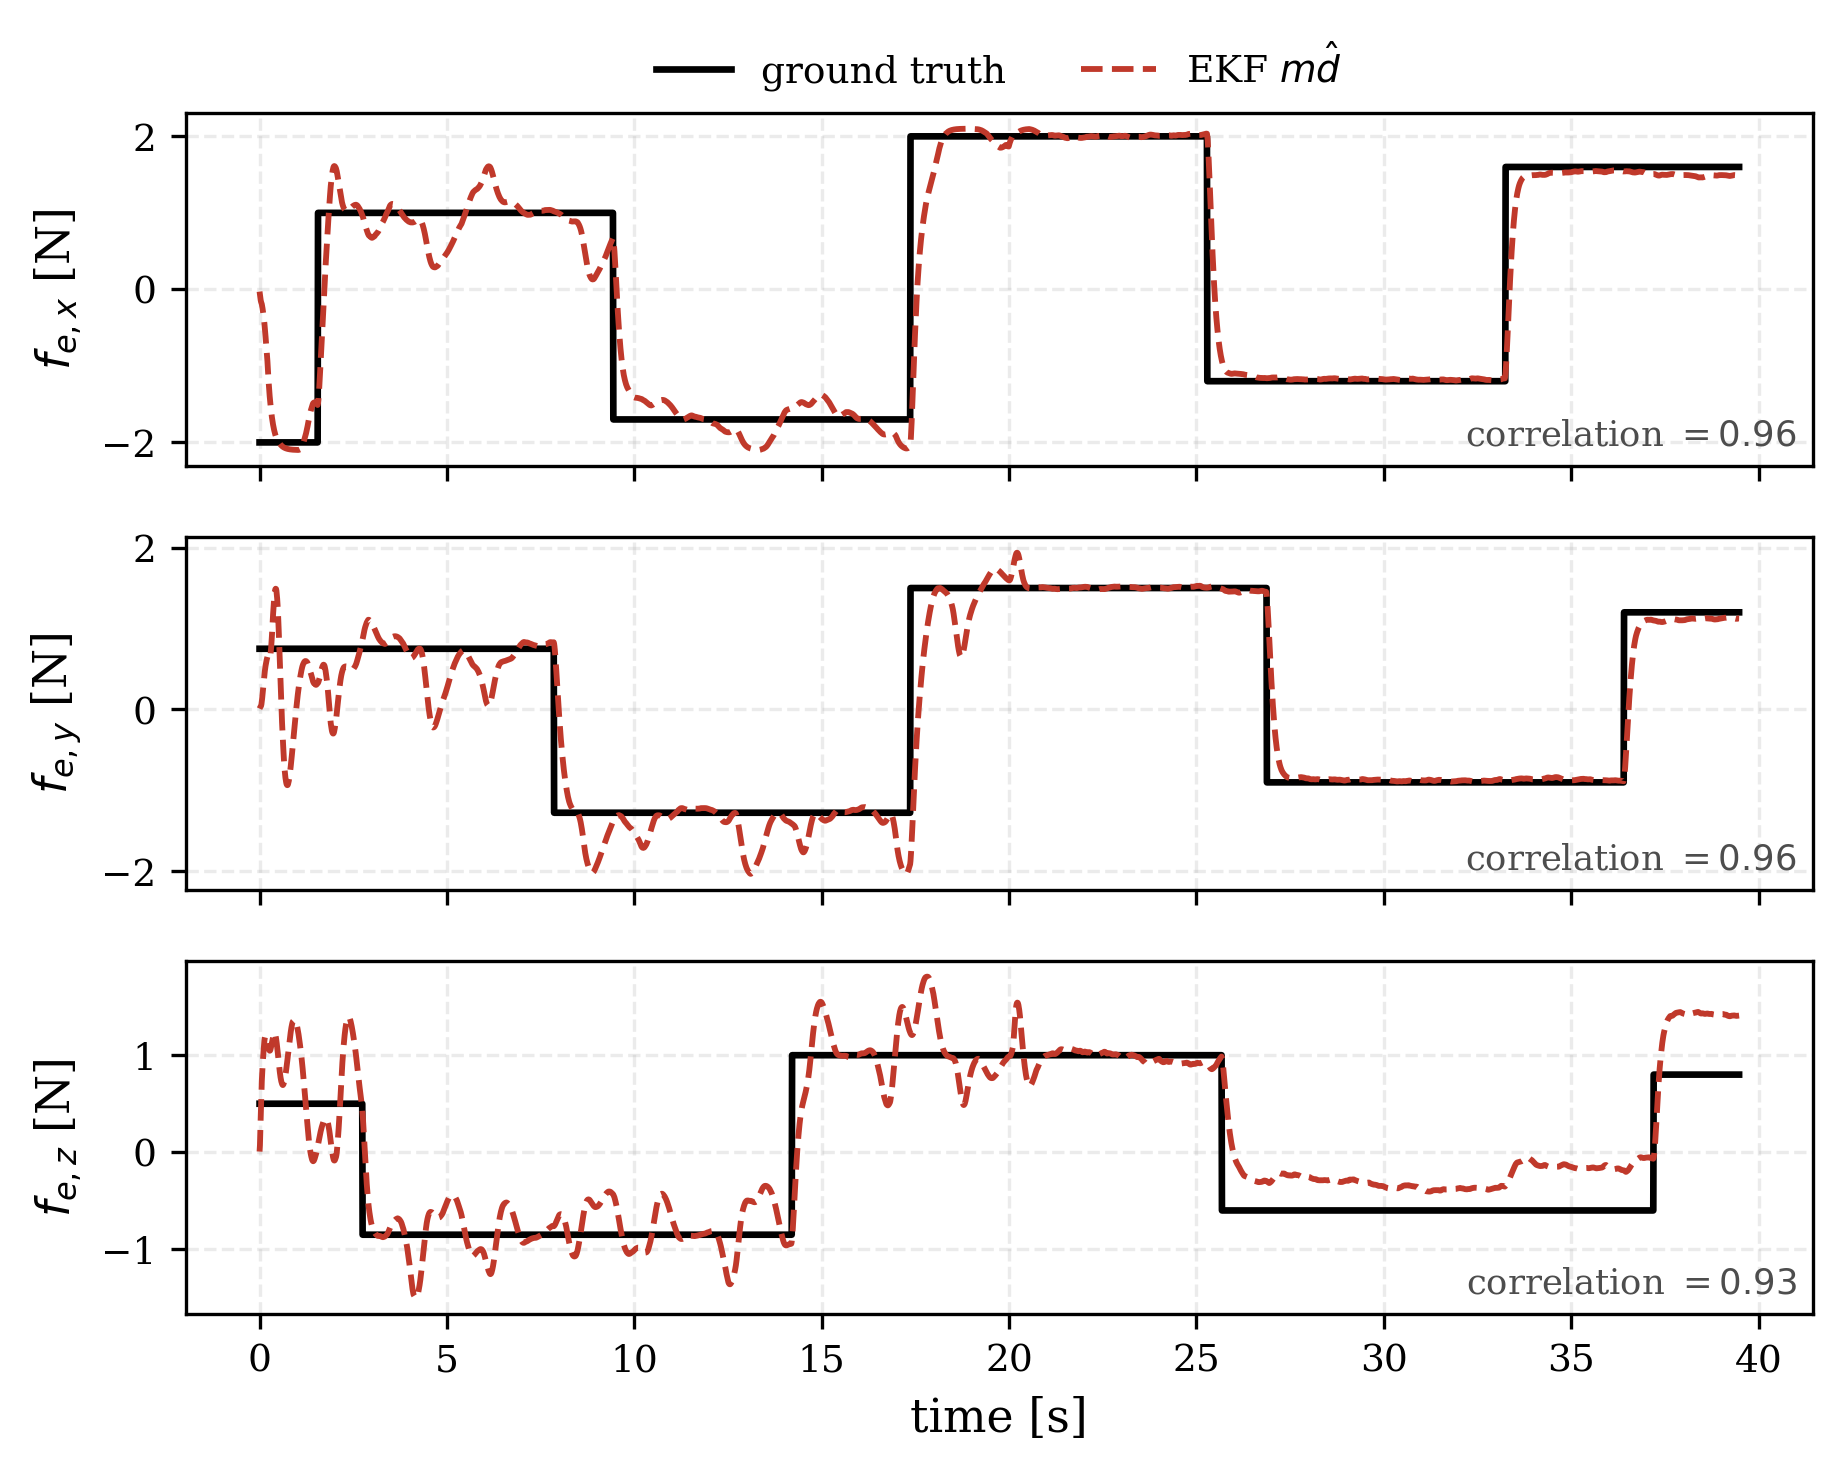
\includegraphics[width=\columnwidth]{figs/fig_dhat.png}
\caption{Virtual force sensor in the time domain (representative run):
$m\hat{\vect{d}}$ tracks the applied wind steps on all three axes.}
\label{fig:dhat}
\end{figure}

\begin{figure}[t]
\centering

\includegraphics[width=\columnwidth]{figs/fig_force_corr.png}
\caption{Per-axis force correlation against excitation ($N{=}10$; $9$ in hover;
step ground truth).}
\label{fig:force}
\end{figure}

We characterize the sensor with a calibration curve, the standard test for a force
sensor: the estimated force ($m\hat{\vect{d}}$) against the applied force, per axis,
over a sinusoidal wind that sweeps the range (Fig.~\ref{fig:calib}). The fit is
linear and correctly scaled, with slopes \num{0.98}, \num{0.97}, \num{0.96} for the three axes,
sub-\SI{0.2}{\newton} intercepts, and $R^2$ of \num{0.90}, \num{0.89}, \num{0.87};
the unity slope confirms the reading is correctly scaled by the mass and the small
residual is the bandwidth limit of the random-walk force model. The sensor is
bandwidth-limited rather than range-limited: an amplitude sweep of step disturbances
shows the slope holding above \num{0.8} up to about \SI{2}{\newton} and then falling
(to \num{0.4} at \SI{4}{\newton}) as large, fast steps exceed the random-walk
bandwidth, so the usable full scale is set by how quickly the disturbance varies, a
limitation a higher-order force model would relax.

\begin{figure}[t]
\centering
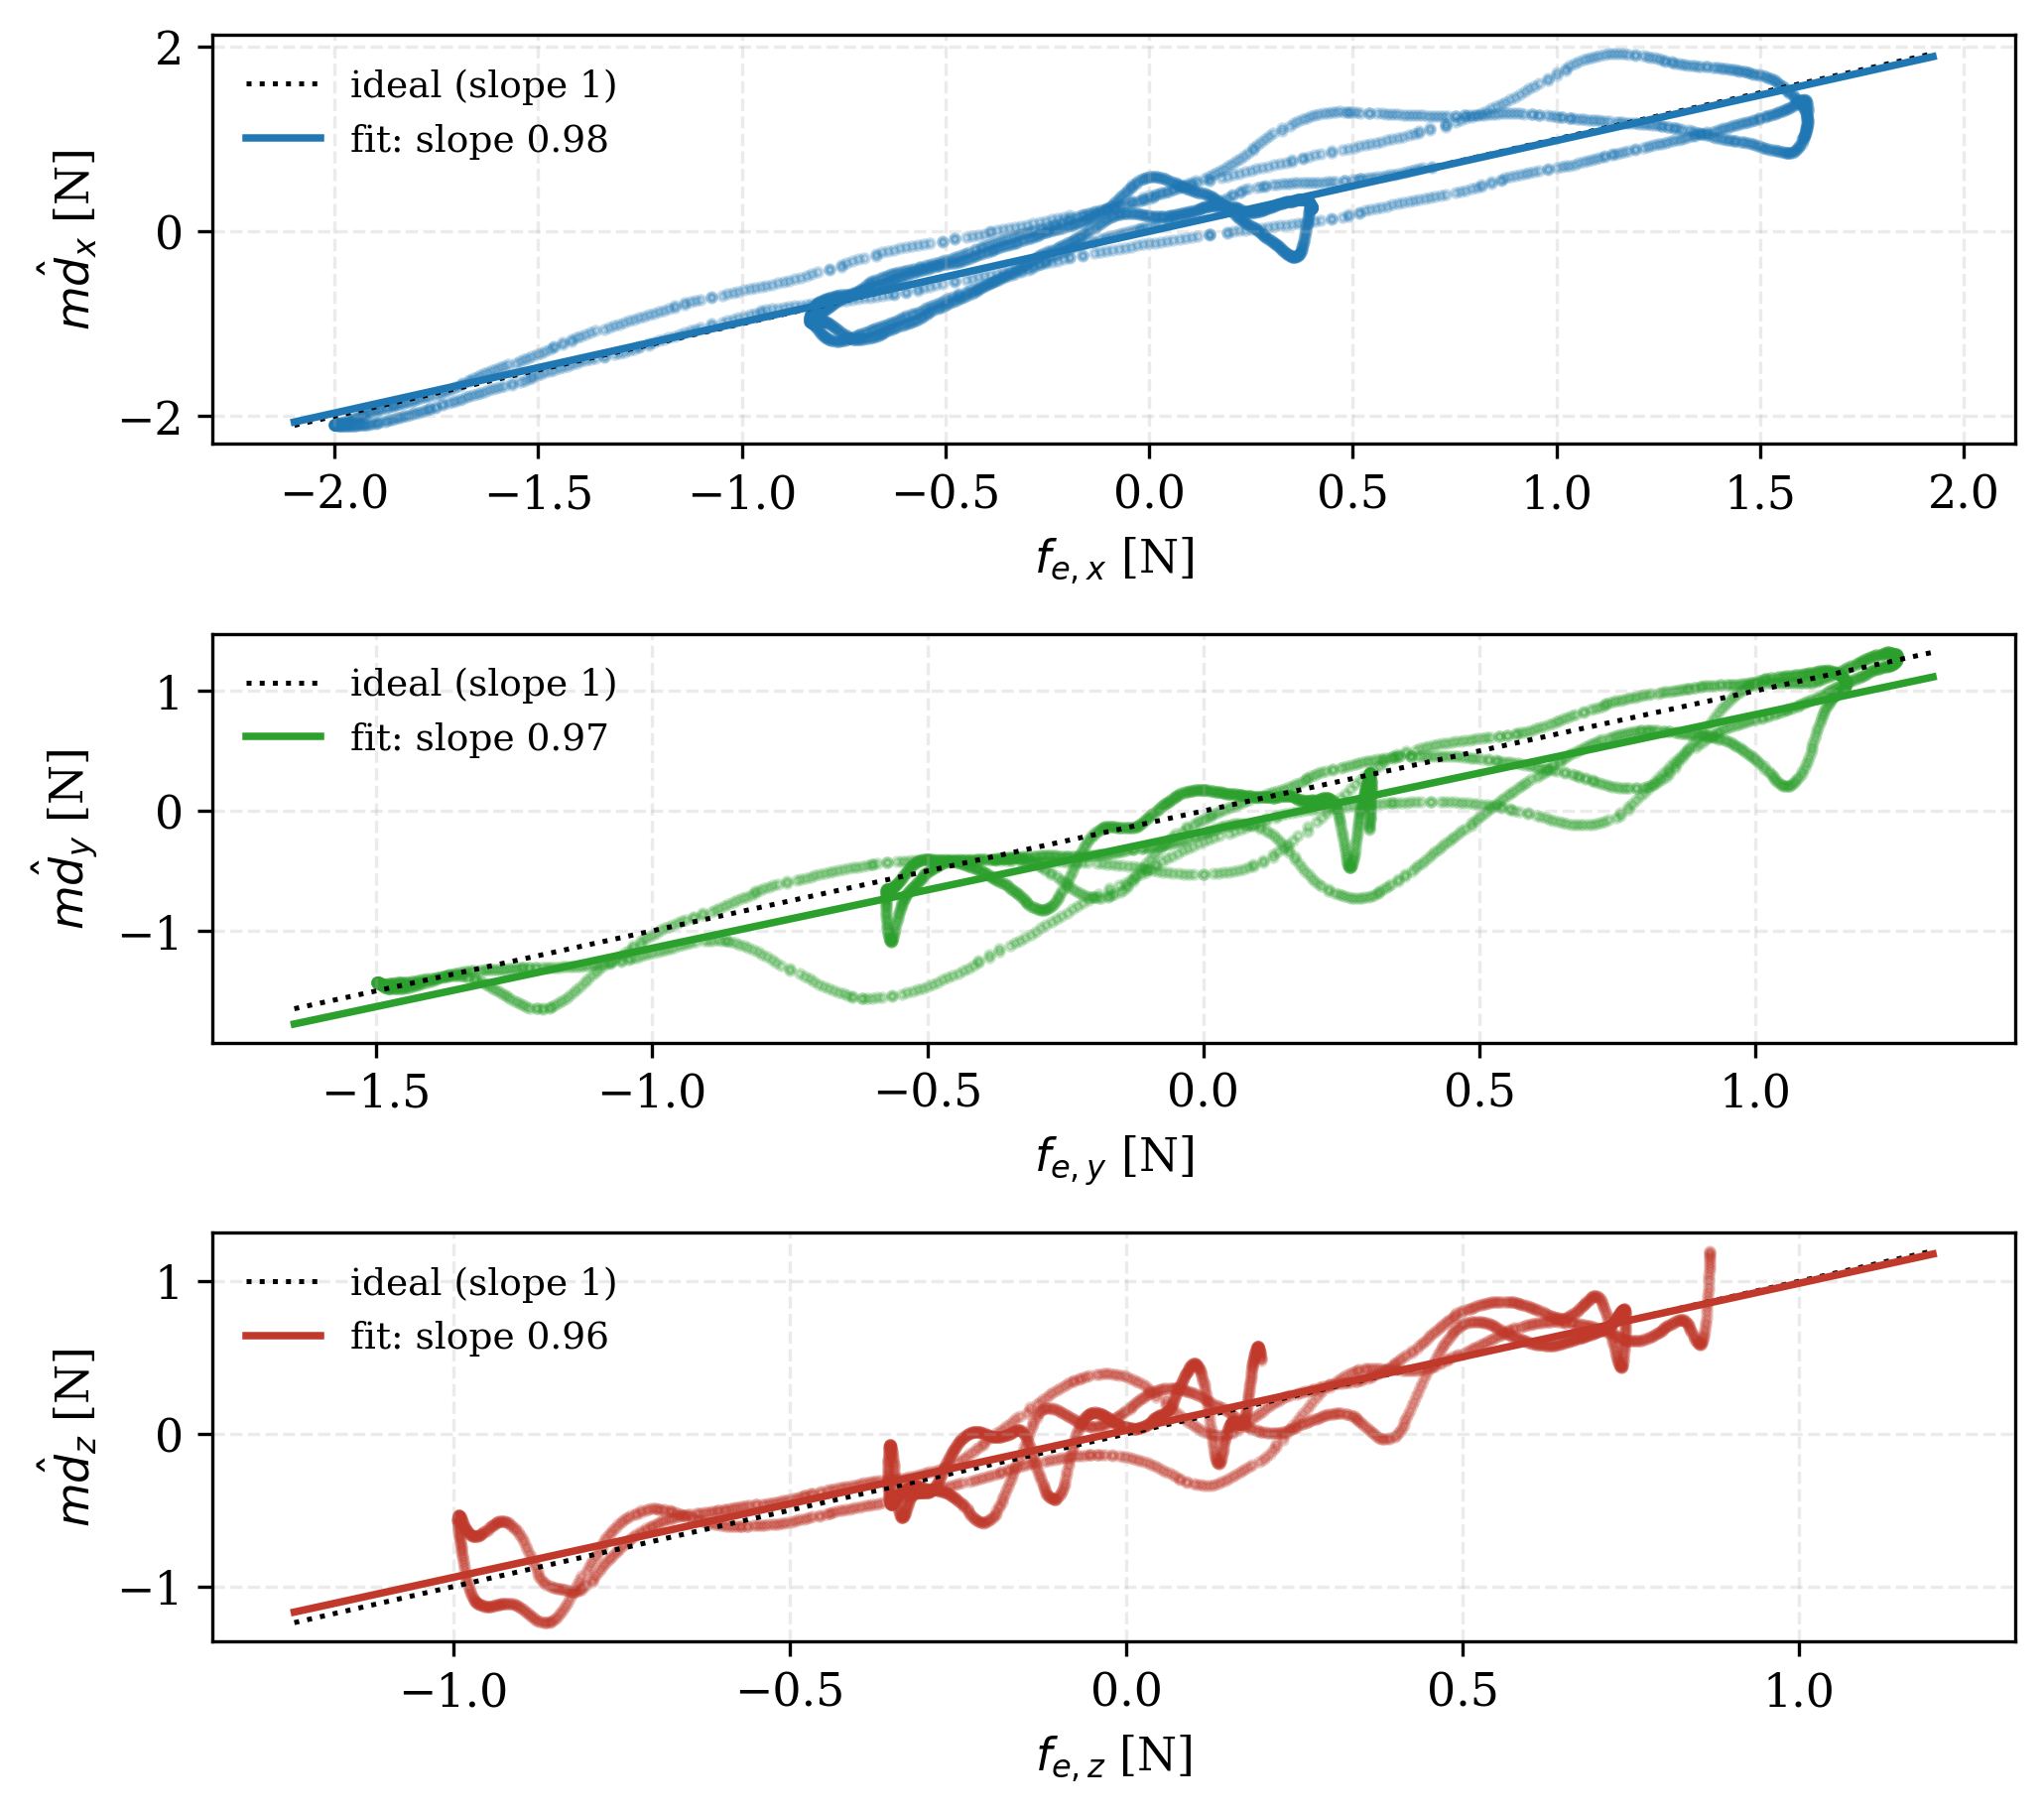
\includegraphics[width=\columnwidth]{figs/fig_calib.png}
\caption{Calibration curve under a sinusoidal wind: estimated force against
applied force for, from top to bottom, the $x$, $y$, and $z$ axes, with the linear fit
(slopes \num{0.98}, \num{0.97}, \num{0.96}; $R^2$ \num{0.90}, \num{0.89},
\num{0.87}) and the ideal unit slope.}
\label{fig:calib}
\end{figure}

\subsection{Mass identification and its hover limit}
Given excitation and no confounding disturbance, the mass is identified
accurately: Fig.~\ref{fig:massconv} shows the EKF converging from a deliberately
wrong prior (\SI{0.60}{\kilogram}, \SI{43}{\percent} low) to within
\SI{0.6}{\percent} of the ground truth on a disturbance-free trajectory, with the
estimated force correctly near zero. This is the identification result: the mass
is a physical invariant and is recovered to the true value once the trajectory
disperses the thrust vector.

\begin{figure}[t]
\centering

\includegraphics[width=\columnwidth]{figs/fig_massconv.png}
\caption{Mass identification under excitation: from a \SI{0.60}{\kilogram} prior
to within \SI{0.6}{\percent} (disturbance-free trajectory).}
\label{fig:massconv}
\end{figure}

Hover is where identification is hard, and it exposes the limit of the ungated
filter: Fig.~\ref{fig:mass} shows the plain EKF mass against speed under wind
\emph{without} the gate: in hover the estimate is biased by \SI{4.8}{\percent} and
varies by $\pm\SI{35}{\gram}$ across the $N=9$ runs, because the vertical force is
misread as a mass change (Proposition~\ref{prop:hover}); under excitation the bias
falls below \SI{1}{\percent} and the spread to $\pm\SI{2}{\gram}$, in agreement
with the $\sigma^{-1}$ conditioning of Section~\ref{sec:obs}. This hover bias,
which appears even when the mass is seeded from the correct value, is exactly what
the gate prevents, as the next experiment shows.

\begin{figure}[t]
\centering
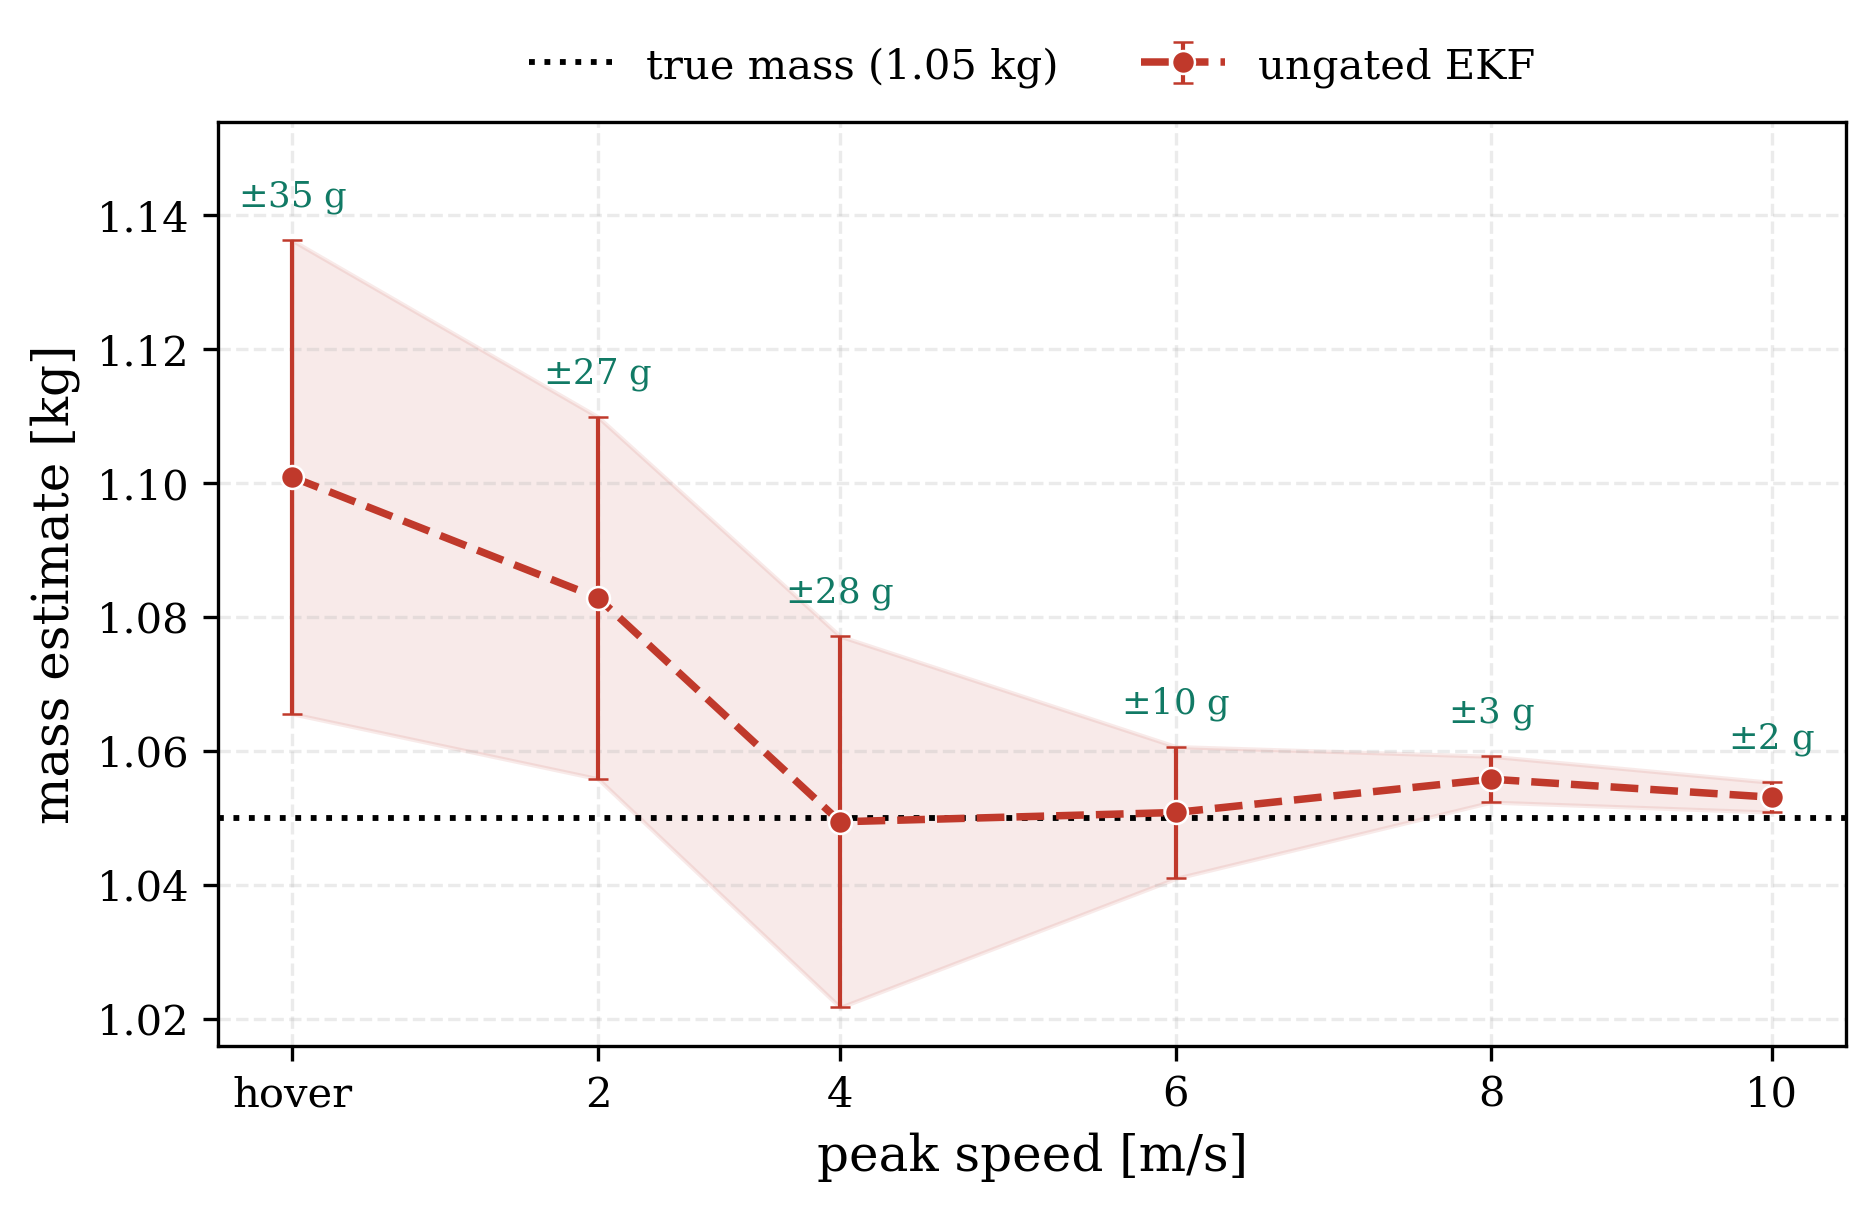
\includegraphics[width=\columnwidth]{figs/fig_mass_id.png}
\caption{Mass identifiability against excitation, \emph{ungated} EKF ($N{=}10$ per
speed, $N{=}9$ in hover; mean $\pm$ std).}
\label{fig:mass}
\end{figure}

\subsection{The mass gate protects the estimate}
The experiment of Fig.~\ref{fig:trans} flies an aggressive trajectory followed by a hover, both
under wind, over five runs with independent noise and wind. During the trajectory
both filters identify the mass. In the hover that follows, the plain EKF is blind
to the lost identifiability and attributes the vertical wind to a mass change; its
drift is more pronounced here than in the steady-hover battery of
Fig.~\ref{fig:mass} (\SI{4.8}{\percent}), because the maneuver leaves the filter
with an inflated mass covariance, so the wind moves the estimate by
\SI{\driftPlain}{\percent} over the transition ($7.0\pm0.6$, $N{=}5$). The
identifiability-aware filter detects $\tilde\sigma$ falling below
$\tilde\sigma_{\min}$ and gates the mass update, cutting the drift to
\SI{\driftGated}{\percent} ($3.3\pm0.8$); a residual movement remains because the
windy hover still excites $\tilde\sigma$ intermittently, but the gate more than
halves the error and is consistently better than the plain EKF across all runs.
The gate protects an estimate that hover can no longer fully support.

This advantage comes specifically from the Schur complement, not merely from gating
on excitation. We ran the same filter with the gate keyed instead to a generic
persistency-of-excitation proxy, the total regressor energy $\sum_k\norm{\mat{\Phi}_k}^2$,
a conventional dead-zone. Because hover is high in thrust energy though zero in
dispersion, this proxy never closes and the result coincides with the ungated plain
EKF: on five repetitions the energy-gated and the plain estimates are identical
at the end of the hover (\SIrange{6.4}{8.7}{\percent} drift on a new set of
noise realizations). A generic
excitation measure cannot tell hover from a maneuver. Only $\tilde\sigma$, which measures the dispersion that isolates the
mass--vertical-force coupling, detects the loss of identifiability and protects the
calibration.

\begin{figure}[t]
\centering

\includegraphics[width=\columnwidth]{figs/fig_trans.png}
\caption{Mass over a windy maneuver-to-hover transition ($N{=}5$, mean $\pm$
std); hover shaded, identifiability signal and threshold at the bottom.}
\label{fig:trans}
\end{figure}

\subsection{Active excitation recovers an unidentifiable mass}
When the mass is unknown and the vehicle must hover, no passive estimator can
recover it. The run of Fig.~\ref{fig:active} starts from a deliberately wrong prior
(\SI{0.70}{\kilogram}) in a wind-free hover, the same conditions for the passive
and the active filter. The passive filter stays frozen at the prior,
since hover provides no information (the passive estimate stays at
$-\SI{33.3}{\percent}$ across all $N{=}5$ runs); the active controller injects the
probe of \eqref{eq:probe}, $\tilde\sigma$ rises above the threshold, the gate
opens, and the mass converges from \SI{0.70}{} toward the ground truth; after
\SI{15}{\second} of gate-open time the probe is withdrawn, the gate closes, and the
estimate is held for the remaining \SI{34}{\second} of hover (the slow rise of
$\tilde\sigma$ after withdrawal is the noise-driven thrust jitter of the hover
and stays a factor of two below the threshold). Using the
most informative probe of Section~\ref{sec:probeopt}, the mass error falls from
\SI{33}{\percent} to below \SI{1}{\percent} ($0.4\pm0.2$, $N{=}5$), the same
accuracy the filter reaches on the disturbance-free trajectory of
Fig.~\ref{fig:massconv} (\SI{0.6}{\percent}): fifteen seconds of probe bring
the estimate to the accuracy the trajectory gives. How fast the recovery proceeds
depends on the probe shape, which the next experiment examines.

\begin{figure}[!t]
\centering

\includegraphics[width=\columnwidth]{figs/fig_active.png}
\caption{Mass recovery from a wrong prior (\SI{0.70}{\kilogram}) in wind-free
hover ($N{=}5$, mean $\pm$ std): the probe (shaded) raises the identifiability
signal, recovers the mass, is withdrawn after \SI{15}{\second} of gate-open time, and the
estimate holds for the rest of the hover. Unlike the excited trajectory of
Fig.~\ref{fig:massconv}, hover provides no information: the passive filter stays
at the prior.}
\label{fig:active}
\end{figure}

\subsection{Shaping the probe by identifiability}\label{sec:probeopt}
The speed of the recovery in Fig.~\ref{fig:active} depends on the probe shape,
and the identifiability tells us which shape is best: since the Schur complement
is the Fisher information on the mass (Proposition~\ref{prop:crb}), the probe
that raises it most per unit deviation tightens the bound fastest. We sweep the
vertical/lateral mix of \eqref{eq:probe} at the fixed amplitude budget
$\rho=\SI{0.8}{\meter}$, from a pure lateral tilt to a pure vertical bob, and
measure the $\tilde\sigma$ achieved while the probe is active and the time for the
mass error to settle below \SI{2}{\percent} (Fig.~\ref{fig:probeopt}, $N{=}5$ per
shape). The achieved $\tilde\sigma$ rises monotonically from \num{0.033} for the
lateral tilt to \num{0.048} for the vertical bob, and the settling time falls in
the same order, from $14.3\pm1.3$ to $8.3\pm0.6$\,\si{\second} (one-sided
Mann--Whitney against the lateral tilt, $p=0.004$), consistent with
Proposition~\ref{prop:crb}: the information rate sets how quickly the bound
tightens. All five shapes exceed the threshold at this budget and all recover the
mass to \SIrange{0.4}{1.2}{\percent}, since the probe is withdrawn only after
\SI{15}{\second} of gate-open time whatever its shape. The ranking is the
opposite of the one we obtained with a preliminary \SI{0.4}{\meter} budget,
where only the lateral tilt exceeded the threshold and the vertical bob
raised $\tilde\sigma$ least, because the controller attenuates a commanded
\SI{1}{\hertz} bob of that amplitude: what counts is the $\tilde\sigma$ the closed
loop actually achieves, not the one the reference prescribes. This is the practical reason for shaping the probe by the
measured $\tilde\sigma$ rather than by a fixed rule, and the shape is optimal only
within the two-parameter family we sweep, not the unconstrained optimal input.

\begin{figure}[t]
\centering
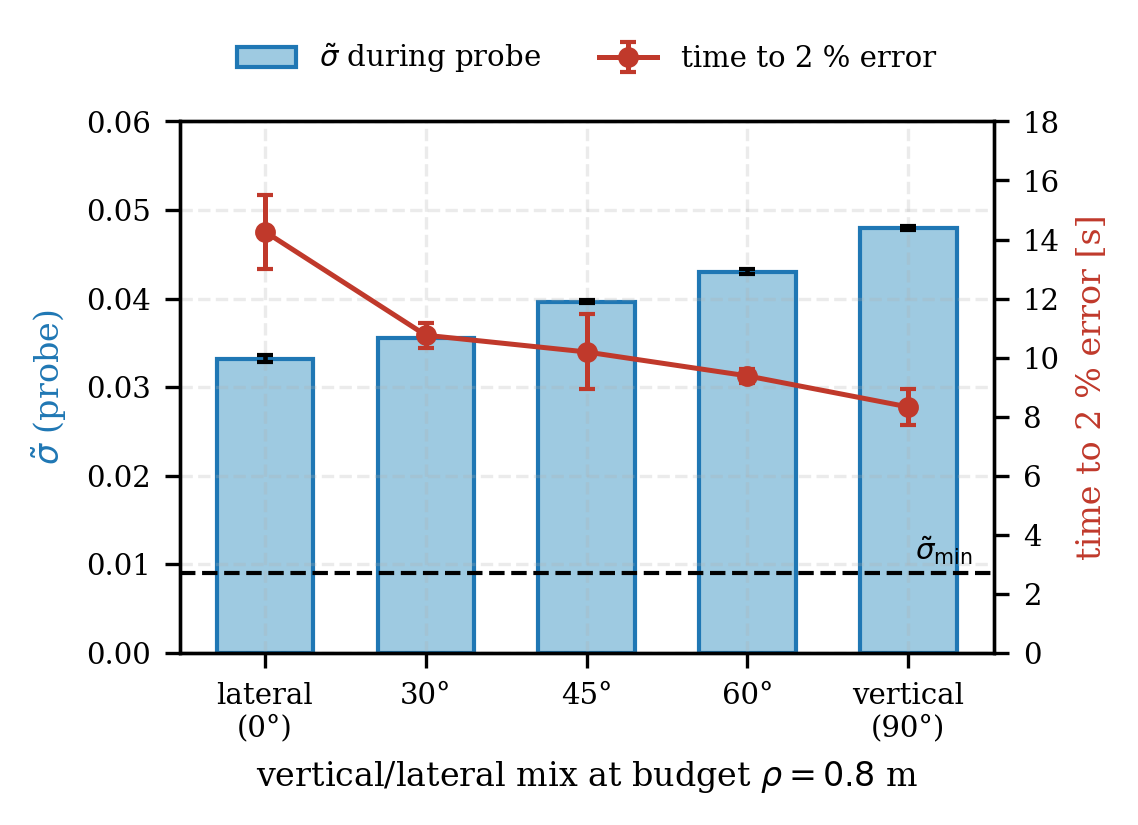
\includegraphics[width=\columnwidth]{figs/fig_probe_opt.png}
\caption{Probe shaping at the \SI{0.8}{\meter} budget: identifiability achieved
while the probe is active (bars) and time for the mass error to settle below
\SI{2}{\percent} (line), against the vertical/lateral mix ($N{=}5$ per shape,
mean $\pm$ std).}
\label{fig:probeopt}
\end{figure}

\subsection{Disturbance rejection}
Feeding the estimated force to the controller reduces the tracking error under
wind (Fig.~\ref{fig:traj}), and the reduction scales with how much the wind
dominates the dynamics (Fig.~\ref{fig:rej}, Table~\ref{tab:rej}). Up to \SI{6}{\meter\per\second} the
wind dominates and the feedforward cuts the error by \SI{77}{} to
\SI{80}{\percent} (\SI{78}{\percent} in hover); as the speed grows the wind
becomes a small fraction of the aerodynamic forces and the reduction falls to
\SI{34}{\percent} at \SI{10}{\meter\per\second}. The improvement is statistically
significant at every speed: a one-sided Mann--Whitney $U$ test of the
feedforward against the baseline rejects the null at each operating point
($p<0.01$, $n=5$ per condition; $p=0.008$ for the $n=4$ hover case), with a large
pooled effect size (Cohen's $d=5.7$). The estimator
and controller each run at \SI{100}{\hertz} with a per-step time below
\SI{1}{\milli\second} on the processor of Section~\ref{sec:nmpc}. The spatial effect on the figure-eight is shown in
Fig.~\ref{fig:traj}: with the feedforward the vehicle stays on the reference, while
without it the wind pushes it off the path.

\begin{figure}[t]
\centering

\includegraphics[width=\columnwidth]{figs/fig_traj.png}
\caption{Trajectory under wind: with the feedforward (blue) versus without
(red); reference dotted.}
\label{fig:traj}
\end{figure}

\begin{figure}[t]
\centering
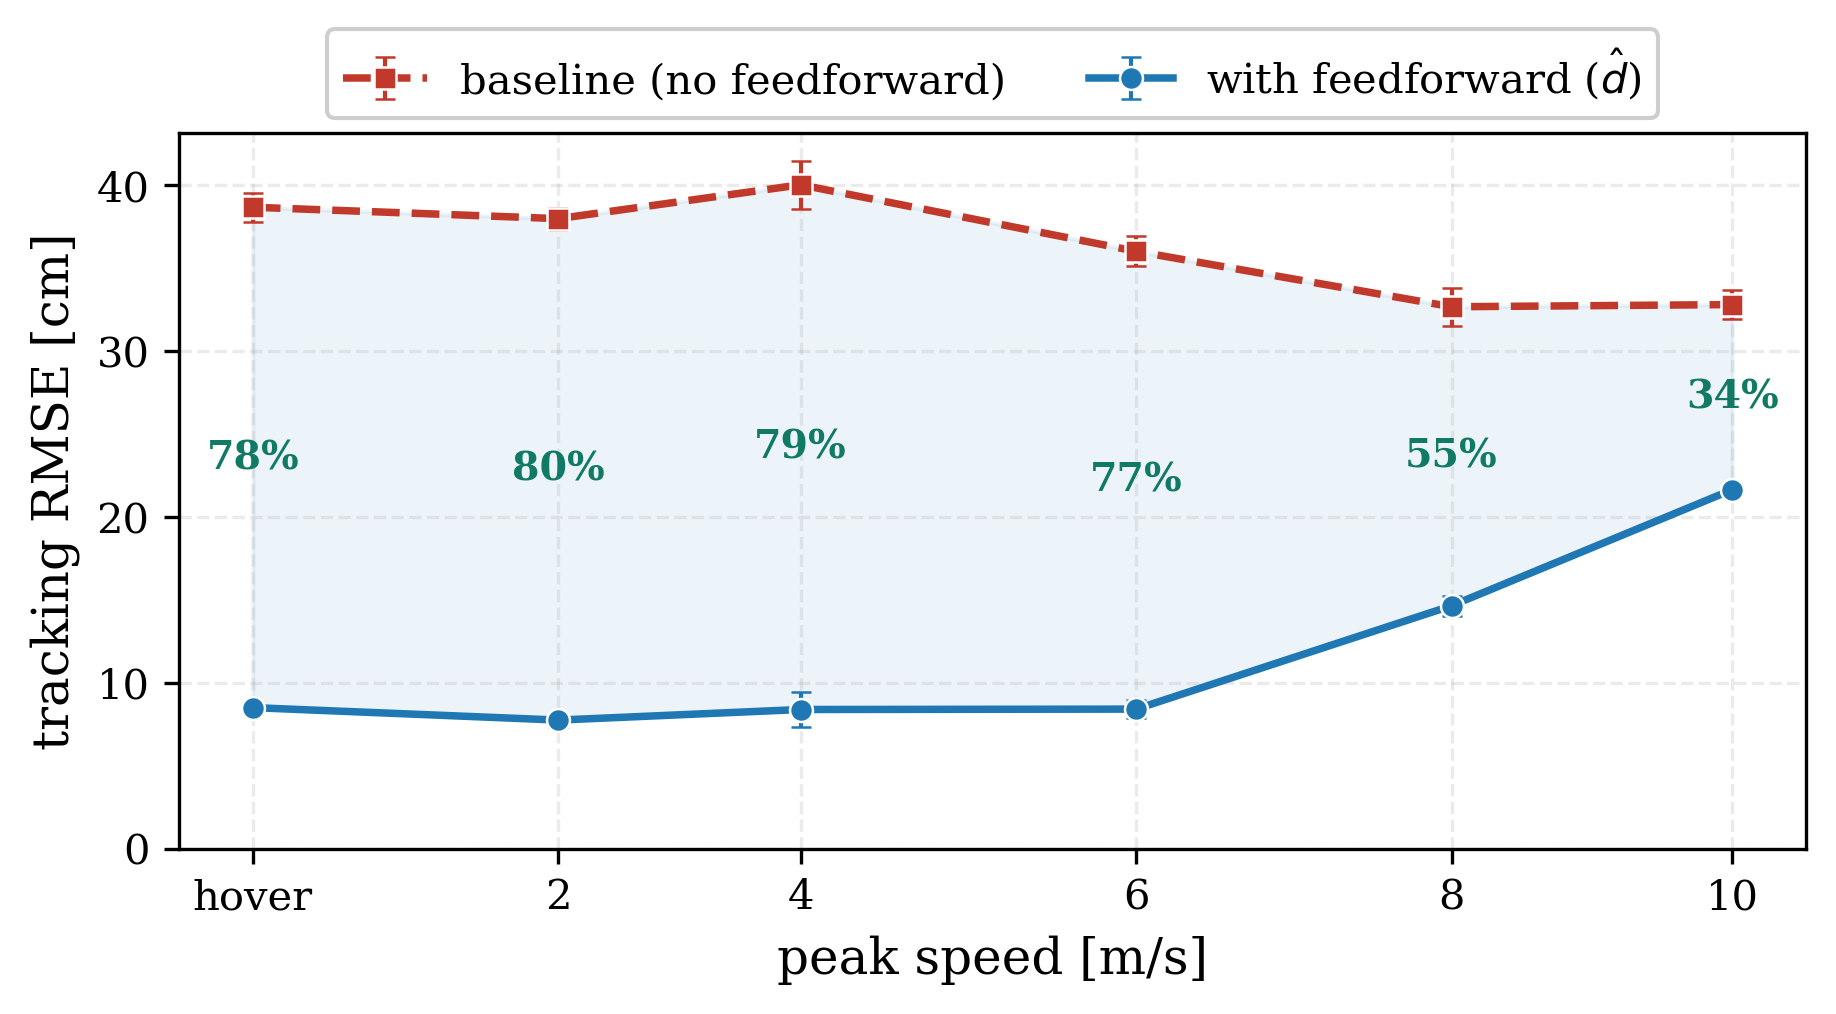
\includegraphics[width=\columnwidth]{figs/fig_rejection.png}
\caption{Disturbance rejection against speed ($N{=}5$ per mode; hover $N{=}4$;
mean $\pm$ std).}
\label{fig:rej}
\end{figure}

\begin{table}[t]
\centering
\caption{Disturbance rejection ($N=5$ per mode; hover $N=4$): tracking RMSE with and without the force
feedforward under the same wind, against peak speed.}
\label{tab:rej}
\begin{tabular}{cccc}
\toprule
Peak [\si{\meter\per\second}] & No ff [\si{\centi\meter}] & ff [\si{\centi\meter}] & Reduction \\
\midrule
hover & $38.7$ & $8.5$  & $78\%$ \\
2.1   & $38.0$ & $7.8$  & $80\%$ \\
3.8   & $40.0$ & $8.4$  & $79\%$ \\
6.1   & $36.0$ & $8.4$  & $77\%$ \\
8.2   & $32.7$ & $14.6$ & $55\%$ \\
10.2  & $32.8$ & $21.6$ & $34\%$ \\
\bottomrule
\end{tabular}
\end{table}

\subsection{Robustness}\label{sec:robust}
The virtual force sensor is not specific to the step disturbance used above.
Under a sinusoidal wind, a continuously varying profile, the estimate tracks the
ground truth with a per-axis correlation near \num{0.93} (Fig.~\ref{fig:sine}),
slightly below the step value because the moving disturbance has more bandwidth.
All results so far use the simulator's injected odometry noise, so the estimator
is already exercised on noisy measurements rather than a clean ground-truth
state. The gate threshold is stable across maneuvers once the identifiability is
normalized. The raw $\sigma$ separates the regimes but its absolute scale follows
the thrust level, so it required a maneuver-specific threshold (a span of more
than an order of magnitude across our experiments). The dimensionless
$\tilde\sigma$ of \eqref{eq:snorm} removes that dependence: hover sits at
$\tilde\sigma\approx0.002$ (steady hover, still or windy: Fig.~\ref{fig:active}
and Table~\ref{tab:info}) to \num{0.005} (the post-maneuver windy hover of
Fig.~\ref{fig:trans}, \SI{1}{\second} window median) while the fastest trajectory
reaches \num{0.46} (Table~\ref{tab:info}),
two orders of magnitude apart. A single $\tilde\sigma_{\min}=0.009$ classifies
hover, maneuver, and the active probe alike: the probe lifts $\tilde\sigma$ to
\numrange{0.033}{0.048}, four to five times the threshold (Table~\ref{tab:info}),
while hover keeps the gate closed. How far the threshold, the window, the dwell, the
process and measurement noise, and the maneuver intensity can move before the
gate degrades is quantified in Section~\ref{sec:sens}.

\begin{figure}[t]
\centering
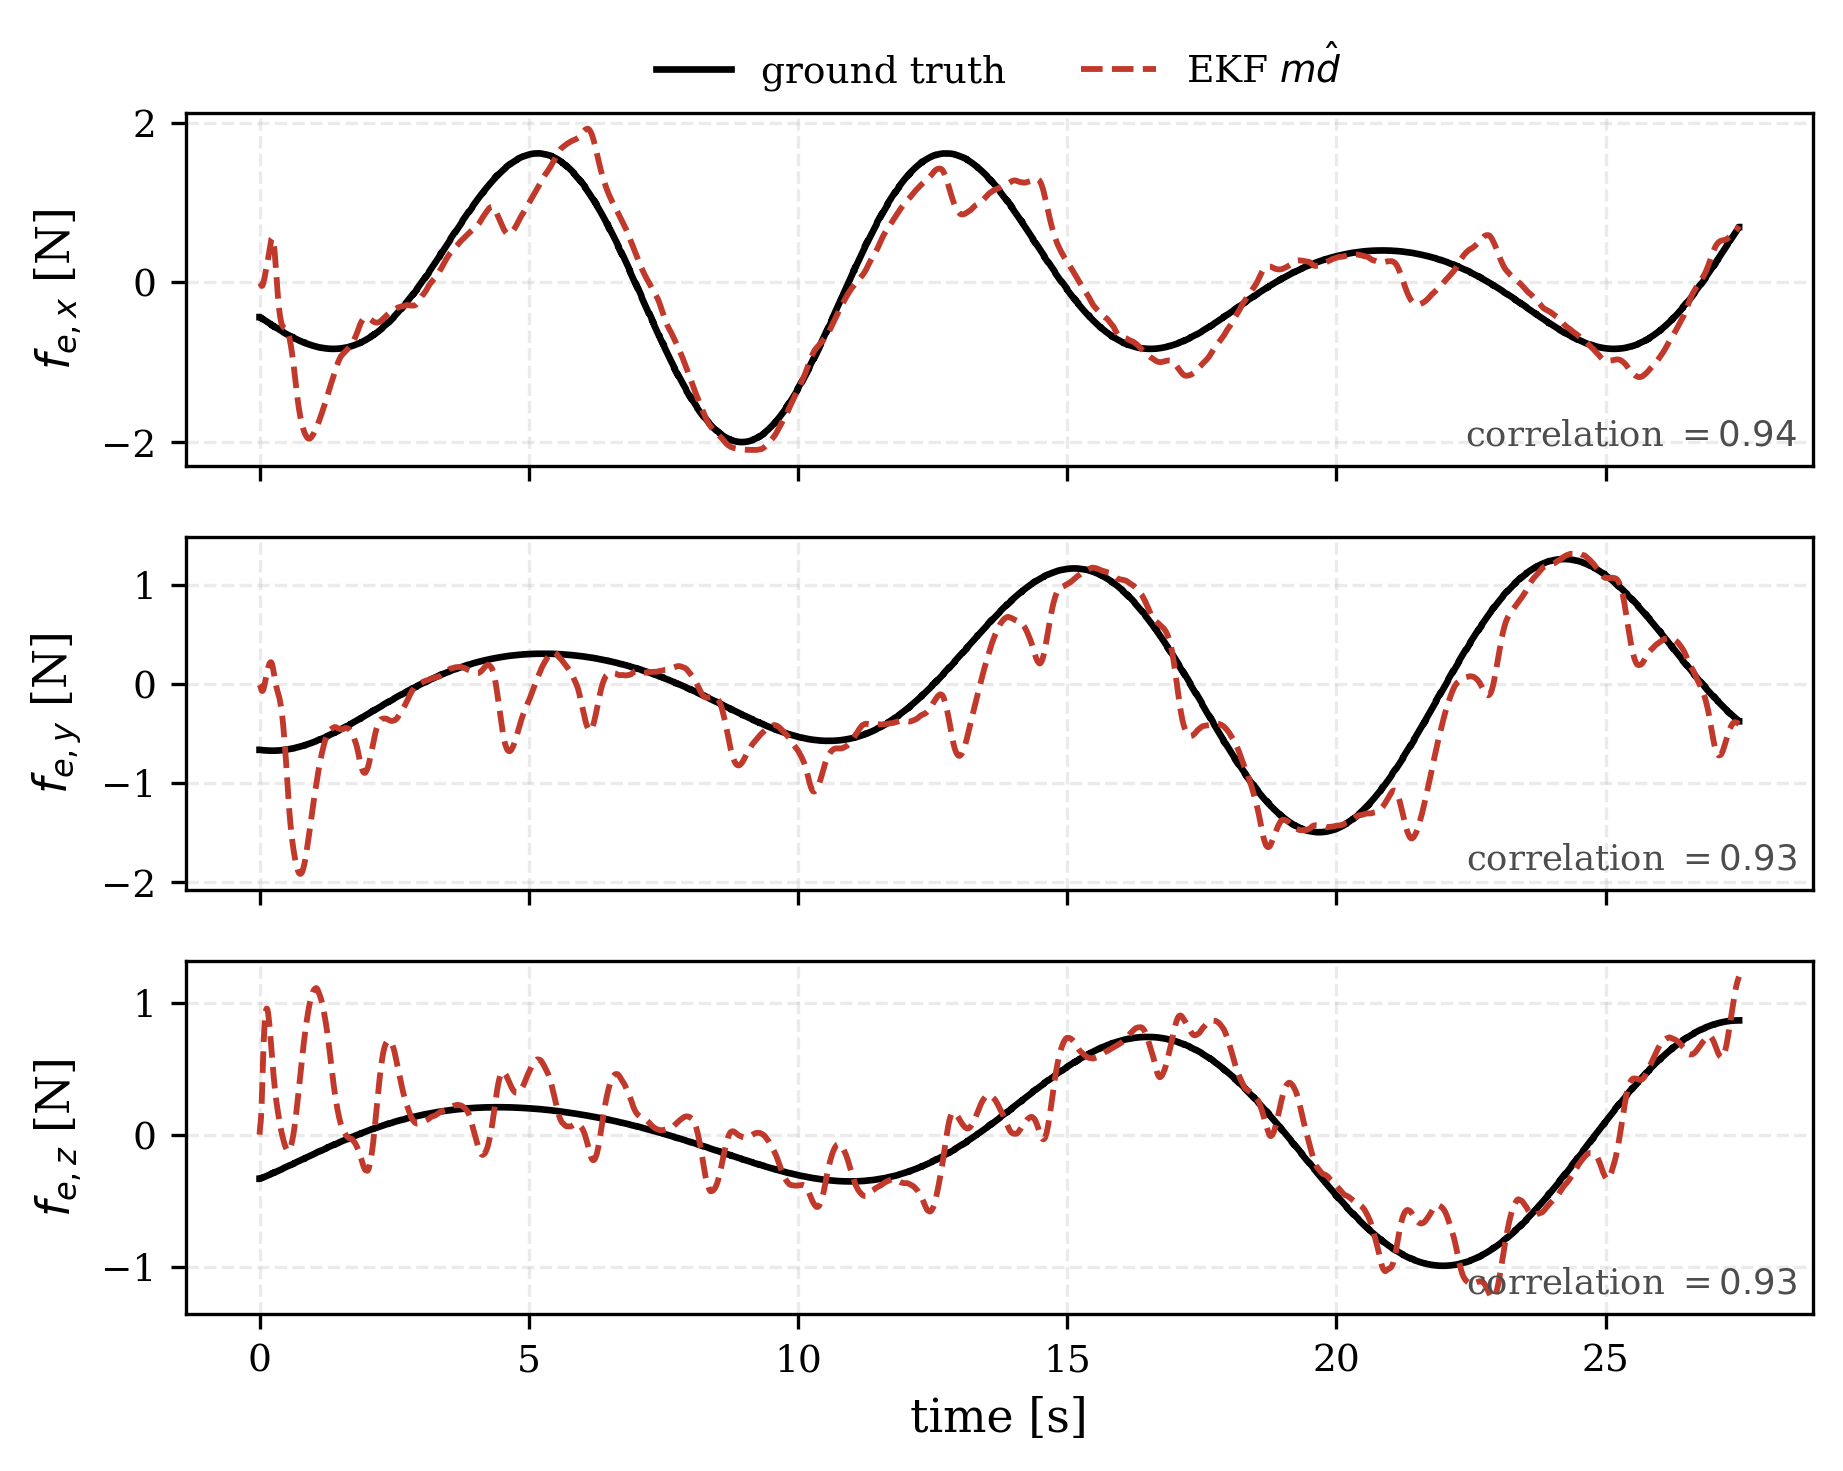
\includegraphics[width=\columnwidth]{figs/fig_dhat_sine.png}
\caption{Virtual force sensor under a sinusoidal wind (representative run);
per-axis correlation near \num{0.93}.}
\label{fig:sine}
\end{figure}

\subsection{Robustness to sensor errors}\label{sec:senserr}
A virtual force sensor lives or dies by the error sources a real IMU and thrust map
introduce, which the ideal simulator does not exercise. We inject them into the
estimator inputs and sweep their magnitude (Fig.~\ref{fig:robust}): an
accelerometer bias up to \SI{0.4}{\meter\per\square\second}, a scale-factor error
up to \SI{10}{\percent}, and a thrust-coefficient mismatch up to \SI{10}{\percent}.
The ranges are chosen to bracket what a real platform presents before any
in-field calibration: the bias range covers the uncalibrated initial offset of
consumer MEMS accelerometers (tens of \si{\milli g}, i.e.\ a few tenths of
\si{\meter\per\square\second}), the scale-factor range covers their sensitivity
tolerance of a few percent with a wide margin, and the thrust range covers the
change of the thrust map over a flight from battery-voltage sag and propeller
wear, which is of the order of \SI{10}{\percent}.
The sensor degrades gracefully and proportionally, with no breakdown. The force
error rises from \SI{0.42}{\newton} to at most \SI{0.58}{\newton} (under the largest
bias), and the mass calibration from below \SI{1}{\percent} to at most
\SI{11.5}{\percent} (under a \SI{10}{\percent} thrust mismatch, which couples almost
one-to-one into the mass). The bias loads the force but barely the mass, while the
scale and thrust errors load the mass through the $\tfrac{T}{m}$ term, as expected; the
near-linear degradation suggests that a one-time bench calibration of the bias
and scale may remove much of it, which we have not tested.

\begin{figure}[t]
\centering
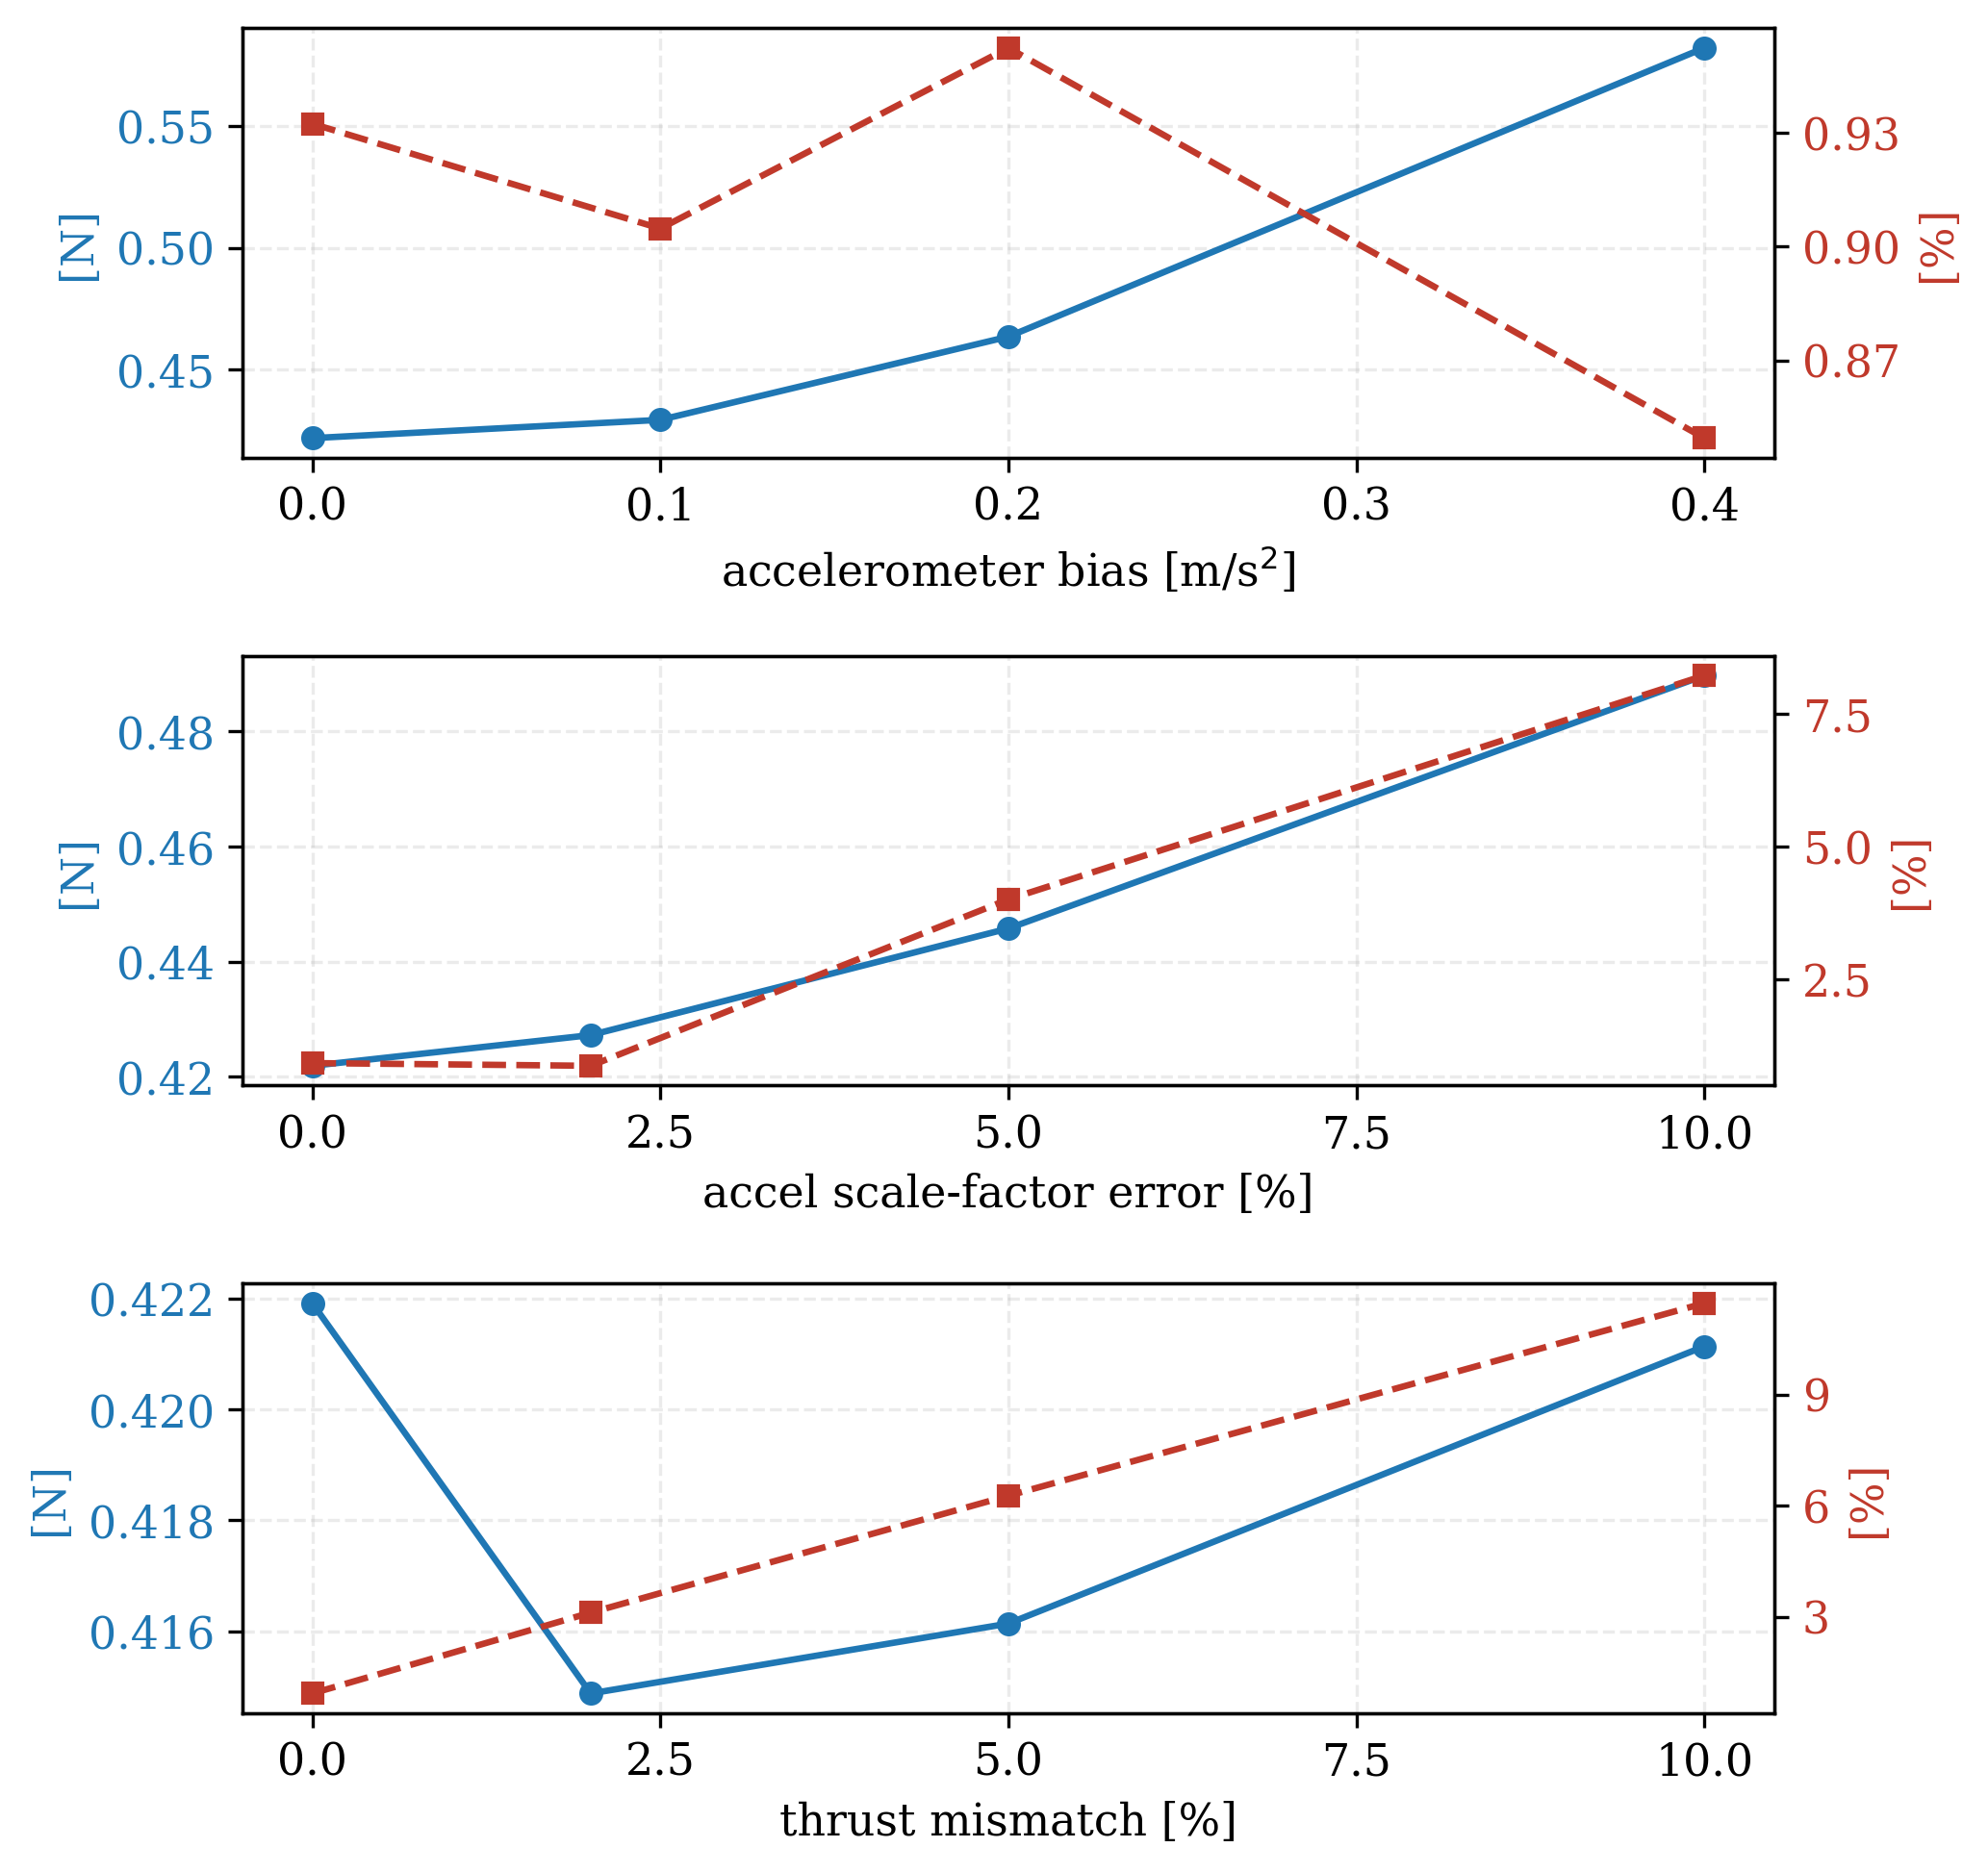
\includegraphics[width=\columnwidth]{figs/fig_robust.png}
\caption{Robustness to injected accelerometer bias, scale-factor error, and
thrust mismatch: force error (blue, left axis) and mass error (red, right
axis).}
\label{fig:robust}
\end{figure}

\subsection{Fisher information, threshold, and gate sensitivity}\label{sec:sens}
Proposition~\ref{prop:crb} bounds the variance of the mass estimate; we check it
against the spread actually observed and then examine how sensitive the gate is
to its parameters. To this end, Fig.~\ref{fig:fisher}(a) plots, against speed, the across-run
standard deviation of the plain-EKF mass from Table~\ref{tab:id} together with
the constant-force bound of Proposition~\ref{prop:crb} and the random-walk bound
of \eqref{eq:sigeff}, both computed from the logged thrust and attitude with
the filter's $r_s$ and $q_d$ and accumulated over the full run (unlike the
per-window values of Table~\ref{tab:info}); the random-walk information over a
\SI{1}{\second} window is \SI{12}{\percent} of the constant-force value at the
implemented $q_d$ (Fig.~\ref{fig:fisher}(b)). Under excitation (\SIrange{6.1}{10.2}{\meter\per\second})
the empirical spread falls from \SI{10}{} to \SI{2.2}{\gram} while the
constant-force bound falls from \SI{2.4}{} to \SI{0.9}{\gram}; scaling by the
random-walk ratio of Fig.~\ref{fig:fisher}(b) brings the bound to
\SIrange{2.5}{7}{\gram}, the scale of the spread (it can even exceed it at the two
fastest speeds, since the across-run spread of a recursive estimate that
accumulates many windows is not the per-window variance the bound addresses), so
the Fisher information of Section~\ref{sec:obs} describes the estimator that is
actually implemented once the force model is accounted for. Near hover the spread
(\SI{35}{\gram}) exceeds both bounds by a wide margin because the error there is a
\emph{bias}, the vertical wind misread as mass, which no variance bound captures:
this is Proposition~\ref{prop:hover} seen from the estimator side and the reason
the gate is needed.

\begin{figure}[t]
\centering

\includegraphics[width=\columnwidth]{figs/fig_fisher.png}
\caption{Fisher information on the mass from logged flight data. (a) Across-run
standard deviation of the plain-EKF mass against speed, with the constant-force
bound and the random-walk bound. (b) Ratio of the random-walk to the
constant-force information against window length (\SIrange{0.25}{4}{\second})
for $q_d$ from $0$ to $0.1$ per step.}
\label{fig:fisher}
\end{figure}

Table~\ref{tab:info} separates the two roles of the identifiability signal. The
classification signal $\tilde\sigma$ spans two orders of magnitude from hover to
the fastest trajectory, and the probe sits well above the threshold, as intended.
The information content $\sigma/r_s$ spans three orders of magnitude over the same
regimes because it retains the thrust level; the last column converts it through
Proposition~\ref{prop:crb} into the lower bound on the mass standard deviation
that one second of data could achieve. The probe, at $\tilde\sigma=0.048$, carries per second the information of a
flight between \SI{3.8}{} and \SI{6.1}{\meter\per\second}; because all the
near-hover regimes share the same thrust level, $\tilde\sigma$ and $\sigma/r_s$
rank them identically here, but the table makes explicit that equal
$\tilde\sigma$ at different thrust or noise levels would not mean equal
information.

\begin{table}[t]
\centering
\caption{Classification signal against information content, per regime, over
\SI{1}{\second} windows (median over the runs of Table~\ref{tab:id}; probe:
gate-open windows of Fig.~\ref{fig:active}). Last column: Cram\'er--Rao lower
bound on the mass standard deviation from one window (Proposition~\ref{prop:crb}),
the best resolution the window could give.}
\label{tab:info}
\begin{tabular}{lccc}
\toprule
Regime & $\tilde\sigma$ & $\sigma/r_s$ & CRB std$(\hat m)$ [\si{\gram}] \\
\midrule
hover            & $0.0024$ & $47$    & $160$ \\
\SI{2.1}{\meter\per\second}   & $0.0023$ & $48$    & $160$ \\
\SI{3.8}{\meter\per\second}   & $0.014$  & $298$   & $64$  \\
\SI{6.1}{\meter\per\second}   & $0.12$   & $3413$  & $19$  \\
\SI{8.2}{\meter\per\second}   & $0.30$   & $17330$ & $8.4$ \\
\SI{10.2}{\meter\per\second}  & $0.46$   & $48739$ & $5.0$ \\
probe (vertical bob) & $0.048$ & $1068$ & $34$ \\
\bottomrule
\end{tabular}
\end{table}

The window length and the threshold are coupled, and we quantify the coupling
offline on the transition runs of Fig.~\ref{fig:trans} by recomputing
$\tilde\sigma$ from the logged thrust and attitude for windows of
\SIrange{0.25}{4}{\second}. The ratio between the maneuver and the hover medians
of $\tilde\sigma$ is \num{5} at \SI{0.25}{\second}, \num{15} at
\SI{0.5}{\second}, peaks at \num{28} at the \SI{1}{\second} window used, and
falls to \num{16} and \num{9} at \SI{2}{} and \SI{4}{\second}, because a short
window sees too little of the maneuver and a long one lets the windy hover
accumulate dispersion (its median $\tilde\sigma$ rises from \num{0.0025} at
\SI{0.25}{\second} to \num{0.033} at \SI{4}{\second}). The threshold of
\num{0.009} therefore sits between the two medians, with a margin of about two
on the hover side and more than ten on the maneuver side for windows of
\SIrange{0.5}{1}{\second}, and would
have to be raised for windows of \SI{2}{\second} or longer. Within any window the
windy hover still produces transient spikes (its 95th percentile at
\SI{1}{\second} is \num{0.027}), which is what the dwell rejects.

Table~\ref{tab:sens} reports the sensitivity study proper. Each row repeats
the windy maneuver-to-hover transition of Fig.~\ref{fig:trans} with one
parameter changed at a time, five seeds per setting, and reports the
root-mean-square mass error over the settled hover for the gated and the plain
filter; the reference setting of Table~\ref{tab:params} gives $2.2\pm1.0$
against $5.1\pm1.1$\,\si{\percent} (an RMS over the hover, hence lower than the
end-of-transition values of \SI{3.3}{} and \SI{7.0}{\percent} of
Fig.~\ref{fig:trans}). \emph{Threshold}: below \num{0.009} the
gate re-opens on the windy-hover excursions and its advantage shrinks
(\SIrange{3.4}{3.8}{\percent}); at \num{0.015}, which sits at the level of those
excursions, it opens intermittently with the frozen covariance and becomes
erratic ($5.1\pm2.8$\,\si{\percent}); at \numrange{0.03}{0.06} it stays shut
through the whole hover and holds the mass to \SIrange{0.4}{0.6}{\percent}. The
threshold is therefore limited not by the hover but by what must re-open the
gate: the probe and the slowest flight that should still identify the mass. With the
\SI{0.80}{\meter} budget the probe reaches $\tilde\sigma\approx0.048$
(Table~\ref{tab:info}; a preliminary \SI{0.40}{\meter} budget left it at
the threshold, Section~\ref{sec:probeopt}); with it a threshold of \num{0.03} would be admissible for the probe and would hold
the mass below \SI{1}{\percent}, but it would exclude the
\SI{3.8}{\meter\per\second} flight ($\tilde\sigma=0.014$) from identification, so
we retain \num{0.009} and accept the residual re-openings in windy hover.
\emph{Dwell}: the gate is never worse than the plain filter for dwells of
\SIrange{0.1}{1}{\second} and is best at the \SI{0.25}{\second} used; a short
dwell lets gusts open it too often, and a long one makes re-openings rare but
larger, since each is made with the covariance frozen since the maneuver (the
end-of-hover value at \SI{1}{\second}, not listed in Table~\ref{tab:sens}, scatters
by $\pm7$\,\si{\percent}).
\emph{Window}: \SI{0.5}{\second} is too short to separate the regimes and the
gate degrades to \SI{8.8}{\percent}; \SIrange{1}{2}{\second} hold at
\SIrange{2.2}{3.1}{\percent}. \emph{Process noise}: the gate helps for
$q_m\le10^{-5}$ and is counterproductive at $q_m=10^{-4}$, where a mass that
adapts within a second no longer integrates the hover bias and the plain filter
is already at \SI{3.6}{\percent}. The force process noise sets how much of the
hover ambiguity the filter resolves by fiat: at $q_d=10^{-3}$ the plain filter
attributes the wind almost entirely to the mass and drifts by
\SI{53}{\percent}, which the gate cuts to \SI{6.9}{\percent}; at $q_d=10^{-1}$
the force absorbs everything, the plain filter drifts by only
\SI{1.8}{\percent}, and the gate is unnecessary ($4.7\pm2.6$\,\si{\percent}). A
loose force model hides the ambiguity rather than resolving it, and is correct
only if the mass never changes; the gate makes the same decision explicit and
conditional on identifiability, and leaves $q_d$ free to be set for the force
reading. \emph{Accelerometer noise}: added white noise of
\SIrange{0.3}{0.7}{\meter\per\square\second} leaves the gated error at
\SIrange{2.2}{2.5}{\percent}; the plain filter's own drift shrinks
(\SIrange{1.9}{2.9}{\percent}) because a noisier residual moves the mass less,
so the margin narrows; at \SI{0.3}{\meter\per\square\second} the two are
statistically indistinguishable ($2.5\pm1.1$ against $1.9\pm0.9$). \emph{Maneuver intensity}: at peak speeds of
\SIrange{5.9}{8.4}{\meter\per\second} the picture is unchanged
(\SIrange{2.2}{2.7}{} against \SI{5}{\percent}); at \SI{3}{\meter\per\second}
the maneuver never lifts $\tilde\sigma$ above the threshold, neither filter
identifies the mass, the mass covariance never contracts, and both are
vulnerable to the transient at the hover onset (\SI{44}{\percent} plain,
$40\pm44$\,\si{\percent} gated, one run in five latching a wrong value after a
brief opening). This is the regime the passive gate cannot handle by
construction, since it protects an estimate that was never formed, and the one
the active probe of Section~\ref{sec:active} exists for. The operating region of
the gate is therefore a window of \SIrange{1}{2}{\second}, a dwell of about
\SI{0.25}{\second} (longer dwells keep the RMS error but make the end value
erratic), $q_m\le10^{-5}$, $q_d\le10^{-2}$, and a threshold between the hover
excursions and the probe level, with the probe budget as the lever that widens
it. Transfer to other vehicles, thrust-to-weight ratios, and IMU grades is not
established by one simulated platform; \eqref{eq:thrcrb} provides a necessary
best-case information condition, not a sufficient accuracy guarantee, for
selecting a threshold from $N$, $r_s$, and the desired mass uncertainty.

\begin{table}[t]
\centering
\caption{Gate sensitivity on the windy maneuver-to-hover transition of
Fig.~\ref{fig:trans}: root-mean-square mass error over the hover [\si{\percent}],
mean $\pm$ std over five seeds, for the gated and the plain filter. One parameter
is changed at a time from the reference setting of Table~\ref{tab:params}.}
\label{tab:sens}
\setlength{\tabcolsep}{4pt}
\begin{tabular}{llcc}
\toprule
Parameter & Value & gated & plain \\
\midrule
threshold $\tilde\sigma_{\min}$ & 0.003 & $3.4\pm0.3$ & $4.6\pm0.7$ \\
 & 0.006 & $3.8\pm0.9$ & $4.6\pm0.3$ \\
 & 0.009 (ref.) & $2.2\pm1.0$ & $5.1\pm1.1$ \\
 & 0.015 & $5.1\pm2.8$ & $4.8\pm0.2$ \\
 & 0.03 & $0.4\pm0.3$ & $4.5\pm0.4$ \\
 & 0.06 & $0.6\pm0.2$ & $4.4\pm0.5$ \\
\midrule
dwell $t_d$ [\si{\second}] & 0.1 & $3.5\pm0.9$ & $4.8\pm0.3$ \\
 & 0.25 (ref.) & $2.2\pm1.0$ & $5.1\pm1.1$ \\
 & 0.5 & $4.1\pm1.4$ & $4.4\pm0.8$ \\
 & 1 & $3.1\pm1.6$ & $4.7\pm0.6$ \\
\midrule
window [\si{\second}] & 0.5 & $8.8\pm3.9$ & $4.7\pm0.5$ \\
 & 1 (ref.) & $2.2\pm1.0$ & $5.1\pm1.1$ \\
 & 2 & $3.1\pm0.6$ & $4.7\pm0.4$ \\
\midrule
$q_m$ & $10^{-6}$ & $0.7\pm0.3$ & $1.8\pm0.4$ \\
 & $10^{-5}$ (ref.) & $2.2\pm1.0$ & $5.1\pm1.1$ \\
 & $10^{-4}$ & $7.1\pm2.4$ & $3.6\pm0.5$ \\
\midrule
$q_d$ & $10^{-3}$ & $6.9\pm0.4$ & $52.7\pm0.1$ \\
 & $10^{-2}$ (ref.) & $2.2\pm1.0$ & $5.1\pm1.1$ \\
 & $10^{-1}$ & $4.7\pm2.6$ & $1.8\pm0.7$ \\
\midrule
accel.\ noise [\si{\meter\per\square\second}] & 0 (ref.) & $2.2\pm1.0$ & $5.1\pm1.1$ \\
 & 0.3 & $2.5\pm1.1$ & $1.9\pm0.9$ \\
 & 0.7 & $2.2\pm0.7$ & $2.9\pm0.7$ \\
\midrule
peak speed [\si{\meter\per\second}] & 3.0 & $39.6\pm43.6$ & $44.4\pm2.3$ \\
 & 5.9 (ref.) & $2.2\pm1.0$ & $5.1\pm1.1$ \\
 & 8.4 & $2.7\pm1.2$ & $5.0\pm0.4$ \\
\bottomrule
\end{tabular}
\end{table}

\subsection{Estimator comparison}
Table~\ref{tab:compare} consolidates the comparison on the identical data. The
two baselines fail in different ways, both traceable to the hover ambiguity of
Proposition~\ref{prop:hover}. The plain EKF reads the force well, including the
vertical axis, but lets the hover mass drift as the vertical wind is misread as a
mass change. The moving-horizon estimator is worse: its free mass both corrupts
the vertical force, which it misreads as mass, and drifts in hover (Fig.~\ref{fig:trans}),
and the window adds cost without recovering either. Our identifiability-aware EKF
keeps both: the EKF structure holds the vertical force, and the gate keeps the mass
closest to the truth in the windy hover (\SI{3.3}{\percent}, against
\SI{7.0}{\percent} for the plain EKF and \SI{5.3}{\percent} for the MHE). With
active excitation it is also the only one that recovers the mass from a wrong prior
in hover. All three run in real time at \SI{100}{\hertz}.

\begin{table}[t]
\centering
\caption{Estimator comparison on identical data. Force entries are pooled over
the battery; the excited-mass entries pool the well-excited runs
(8.2--10.2\,\si{\meter\per\second}, $N{=}10$ each speed); hover and recovery
entries are from Figs.~\ref{fig:trans} and~\ref{fig:active}.}
\label{tab:compare}
\begin{tabular}{lccc}
\toprule
 & MHE & plain EKF & gated EKF \\
 &     & (baseline) & (ours) \\
\midrule
horizontal force corr      & 0.96 & 0.97 & 0.97 \\
vertical force corr        & 0.66 & 0.95 & 0.95 \\
mass error, excited        & $+0.4\%$ & $+0.4\%$ & $+0.4\%$ \\
mass error, windy hover    & $5.3\%$ & $7.0\%$ & $\mathbf{3.3\%}$ \\
recover mass, wrong prior  & no & no & yes \\
\bottomrule
\end{tabular}
\end{table}

% ════════════════════ CONCLUSION ════════════════════
\section{Conclusion}\label{sec:conclusion}

We built a self-calibrating virtual force sensor for quadrotors. The external
specific force is read directly from the accelerometer; its only calibration
parameter, the mass, is identifiable only under excitation and is confounded with a
vertical force in hover. We made the calibration identifiability-aware on two levels:
an extended Kalman filter that gates the mass calibration by the online
identifiability $\tilde\sigma$, freezing it when it cannot be seen, and a
model-predictive controller that injects a minimal probe to restore identifiability
when the mass must be recalibrated but the flight lacks the excitation. In
software-in-the-loop the sensor reads the external force to about \SI{0.4}{\newton}
RMS per axis (per-axis correlation \num{0.93} under continuous wind), the gate holds
the mass across a windy hover transition to \SI{3}{\percent} where a plain EKF drifts to
\SI{7}{\percent}, the active probe
recovers the mass from a wrong prior that hover alone cannot identify, and the
force feedforward reduces the tracking error by \SI{34}{} to \SI{80}{\percent}
under wind, scaling with how much the wind dominates the dynamics.

A matched comparison showed that a moving-horizon estimator does not improve on
the EKF for this problem, because the informative measurement is instantaneous;
the contribution therefore lies in the identifiability logic, not in the estimator
class. The dead-zone and the excitation are each classical; what ties them together
is the closed-form Schur complement, the Fisher information on the mass computed from
known signals (its inverse is the Cram\'er--Rao bound), whose dimensionless form
$\tilde\sigma$ drives the gate and the probe from one online scalar, including the
choice of the most informative excitation. The sensitivity study bounds where this holds: the gate helps for windows of
\SIrange{1}{2}{\second}, a dwell of about \SI{0.25}{\second}, a mass process
noise at or below $10^{-5}$, and a force model stiff enough to read the force
($q_d\le10^{-2}$), and it cannot help where the flight never identifies the
mass, which is the regime the probe exists for; the probe, in turn, is shaped by
the identifiability the closed loop actually achieves, which is why it is
measured rather than prescribed. The main
limitation is that the study is in simulation; hardware validation with a
motion-capture system and a calibrated disturbance is the immediate next step, as
is a continuous (rather than family-restricted) optimal-input design.
Because the filter reads any external specific force, the approach extends toward
contact and tether forces, where an identifiability-aware wrench estimate would
support aerial physical interaction~\cite{ollero2022past,augugliaro2013admittance} without a dedicated force sensor.

\section*{Code Availability}
The source code and experiment scripts are openly available at \url{https://github.com/josevarela90/observability-aware}.

\section*{Acknowledgment}
The authors would like to express their gratitude to Universidad Indoamérica for its support of this research through the “Tecnologías de la Industria 4.0 en Educación, Salud, Empresa e Industria” project, and to the Universidad de las Fuerzas Armadas ESPE for supporting this research through the project "Robots Cooperativos para Misiones de Rescate: Percepción, Navegación y Manipulación en Tiempo Real con Sistemas UAV-UGV-Cuadrúpedo”. In addition, special thanks to Bryan Guevara for his technical support in the development of this research.


% ════════════════════ REFERENCES ════════════════════
\bibliographystyle{IEEEtran}
\bibliography{references}

\begin{IEEEbiography}[{
\includegraphics[width=1in,height=1.25in,clip,keepaspectratio]{jose.png}}]{JOSÉ VARELA-ALDÁS} received the master’s degree in control systems from Escuela Superior Politécnica de Chimborazo, and the Ph.D. degree in electronic engineering from the University of Zaragoza. He is an Industrial Engineer with the Universidad Técnica de Ambato. He is currently Director Research and Associate Professor with Universidad Tecnológica Indoamérica, where he is also the research of the MIST Research Center. His research interests include control systems, robotics, the IoT, machine learning, and virtual reality. In 2023, he was recognized as the Best Young Researcher by IEEE Ecuador. In 2024, he served as the President for the IEEE Ecuador Robotics and Automation Society. In 2025, he founded IEEE PUMABOT, the first battlebot league in Ecuador.
\end{IEEEbiography}

\begin{IEEEbiography}[{
\includegraphics[width=1in,height=1.25in,clip,keepaspectratio]{angy.jpg}}]{ANGÉLICA QUITO} is a Research Professor at Universidad Internacional del Ecuador (UIDE), Ecuador, where she serves as Electronics Area Coordinator and Research Coordinator for the Faculty of Digital Engineering and Emerging Technologies. She is a PhD candidate in Engineering at Universidad Nacional de Cuyo (UNCUYO) and holds an M.Sc. in Industrial Engineering and Productivity (EPN), an M.S. in Applied Artificial Intelligence (UISRAEL), and a B.Sc. in Mechatronics Engineering (ESPE). Her research interests include artificial intelligence, computer vision, automation, robotics, and applied engineering prototypes for industrial and societal impact, including a Biomechanical Spine Simulator recognized as \#1 worldwide in WURI 2026 (C2 category). She is also a selected member of CEDIA’s Linkage and Innovation Commission, strengthening technology transfer and academia–industry collaboration.
\end{IEEEbiography}

\begin{IEEEbiography}[{
\includegraphics[width=1in,height=1.25in,clip,keepaspectratio]{Victor.jpeg}}]{Victor H. Andaluz} is an Electronics and Control Engineer from the National Polytechnic School; he was a scholarship holder of the German Institute for Academic Exchange, DAAD, obtaining his Ph.D. in Control Systems Engineering, after studying at the Institute of Automatics of the National University of San Juan, Argentina and at the Institute of Real-Time Systems of the Leibniz University of Hannover-Germany. Currently, he is a professor at the University of the Armed Forces ESPE. His areas of interest are: Robotics, automation, control systems, virtual and augmented reality.
\end{IEEEbiography}

\begin{IEEEbiography}
[{
\includegraphics[width=1in,height=1.25in,clip,keepaspectratio]{alex.png}}]{ Alexandre Santos Brandão}, received the B.S. degree in electrical engineering from the Federal University of Viçosa, Minas Gerais, Brazil, in 2006, the M.Sc. and Ph.D. degrees in electrical engineering from the Federal University of Espírito Santo, Brazil, in 2008 and 2013, respectively, and the Ph.D. degree in control system engineering from the National University of San Juan, San Juan, Argentina, in 2014. He is currently an Associate Professor with the Department of Electrical Engineering, Federal University of Viçosa, Brazil. He has coauthored more than 20 journal articles, two book chapters, and more than 120 conference papers, besides having advised eight M.Sc. and four Ph.D. students. His research interests include nonlinear control of aerial and terrestrial mobile vehicles and control of multi-robot systems.
\end{IEEEbiography}

\EOD

\vfill

\end{document}
